% UCL Thesis LaTeX Template
%  (c) Ian Kirker, 2014
% 
% This is a template/skeleton for PhD/MPhil/MRes theses.
%
% It uses a rather split-up file structure because this tends to
%  work well for large, complex documents.
% We suggest using one file per chapter, but you may wish to use more
%  or fewer separate files than that.
% We've also separated out various bits of configuration into their
%  own files, to keep everything neat.
% Note that the \input command just streams in whatever file you give
%  it, while the \include command adds a page break, and does some
%  extra organisation to make compilation faster. Note that you can't
%  use \include inside an \include-d file.
% We suggest using \input for settings and configuration files that
%  you always want to use, and \include for each section of content.
% If you do that, it also means you can use the \includeonly statement
%  to only compile up the section you're currently interested in.
% You might also want to put figures into their own files to be \input.

% For more information on \input and \include, see:
%  http://tex.stackexchange.com/questions/246/when-should-i-use-input-vs-include


% Formatting rules for theses are here: 
%  http://www.ucl.ac.uk/current-students/research_degrees/thesis_formatting
% Binding and submitting guidelines are here:
%  http://www.ucl.ac.uk/current-students/research_degrees/thesis_binding_submission

% This package goes first and foremost, because it checks all 
%  your syntax for mistakes and some old-fashioned LaTeX commands.
% Note that normally you should load your documentclass before 
%  packages, because some packages change behaviour based on
%  your document settings.
% Also, for those confused by the RequirePackage here vs usepackage
%  elsewhere, usepackage cannot be used before the documentclass
%  command, while RequirePackage can. That's the only functional
%  difference as far as I'm aware.
\RequirePackage[l2, orthodox]{nag}


% ------ Main document class specification ------
% The draft option here prevents images being inserted,
%  and adds chunky black bars to boxes that are exceeding 
%  the page width (to show that they are).
% The oneside option can optionally be replaced by twoside if
%  you intend to print double-sided. Note that this is
%  *specifically permitted* by the UCL thesis formatting
%  guidelines.
%
% Valid options in terms of type are:
%  phd
%  mres
%  mphil
%\documentclass[12pt,phd,draft,a4paper,oneside]{ucl_thesis}
\documentclass[12pt,phd,a4paper,oneside]{ucl_thesis}


% Package configuration:
%  LaTeX uses "packages" to add extra commands and features.
%  There are quite a few useful ones, so we've put them in a 
%   separate file.
% -------- Packages --------

% This package just gives you a quick way to dump in some sample text.
% You can remove it -- it's just here for the examples.
\usepackage{blindtext}

% This package means empty pages (pages with no text) won't get stuff
%  like chapter names at the top of the page. It's mostly cosmetic.
\usepackage{emptypage}

% The graphicx package adds the \includegraphics command,
%  which is your basic command for adding a picture.
\usepackage{graphicx}

% The float package improves LaTeX's handling of floats,
%  and also adds the option to *force* LaTeX to put the float
%  HERE, with the [H] option to the float environment.
\usepackage{float}

% The amsmath package enhances the various ways of including
%  maths, including adding the align environment for aligned
%  equations.
\usepackage{amsmath}
\usepackage{amssymb}

% Use these two packages together -- they define symbols
%  for e.g. units that you can use in both text and math mode.
% \usepackage{gensymb}
% \usepackage{textcomp}
% You may also want the units package for making little
%  fractions for unit specifications.
%\usepackage{units}


% The setspace package lets you use 1.5-sized or double line spacing.
\usepackage{setspace}
\setstretch{1.5}

% That just does body text -- if you want to expand *everything*,
%  including footnotes and tables, use this instead:
%\renewcommand{\baselinestretch}{1.5}


% PGFPlots is either a really clunky or really good way to add graphs
%  into your document, depending on your point of view.
% There's waaaaay too much information on using this to cover here,
%  so, you might want to start here:
%   http://pgfplots.sourceforge.net/
%  or here:
%   http://pgfplots.sourceforge.net/pgfplots.pdf
%\usepackage{pgfplots}
%\pgfplotsset{compat=1.3} % <- this fixed axis labels in the version I was using

% PGFPlotsTable can help you make tables a little more easily than
%  usual in LaTeX.
% If you're going to have to paste data in a lot, I'd suggest using it.
%  You might want to start with the manual, here:
%  http://pgfplots.sourceforge.net/pgfplotstable.pdf
%\usepackage{pgfplotstable}

% These settings are also recommended for using with pgfplotstable.
%\pgfplotstableset{
%	% these columns/<colname>/.style={<options>} things define a style
%	% which applies to <colname> only.
%	empty cells with={--}, % replace empty cells with '--'
%	every head row/.style={before row=\toprule,after row=\midrule},
%	every last row/.style={after row=\bottomrule}
%}


% The mhchem package provides chemistry formula typesetting commands
%  e.g. \ce{H2O}
%\usepackage[version=3]{mhchem}

% And the chemfig package gives a weird command for adding Lewis 
%  diagrams, for e.g. organic molecules
%\usepackage{chemfig}

% The linenumbers command from the lineno package adds line numbers
%  alongside your text that can be useful for discussing edits 
%  in drafts.
% Remove or comment out the command for proper versions.
%\usepackage[modulo]{lineno}
% \linenumbers 


% Alternatively, you can use the ifdraft package to let you add
%  commands that will only be used in draft versions
%\usepackage{ifdraft}

% For example, the following adds a watermark if the draft mode is on.
%\ifdraft{
%  \usepackage{draftwatermark}
%  \SetWatermarkText{\shortstack{\textsc{Draft Mode}\\ \strut \\ \strut \\ \strut}}
%  \SetWatermarkScale{0.5}
%  \SetWatermarkAngle{90}
%}


% The multirow package adds the option to make cells span 
%  rows in tables.
\usepackage{multirow}


% Subfig allows you to create figures within figures, to, for example,
%  make a single figure with 4 individually labeled and referenceable
%  sub-figures.
% It's quite fiddly to use, so check the documentation.
%\usepackage{subfig}

% The natbib package allows book-type citations commonly used in
%  longer works, and less commonly in science articles (IME).
% e.g. (Saucer et al., 1993) rather than [1]
% More details are here: http://merkel.zoneo.net/Latex/natbib.php
%\usepackage{natbib}

% The bibentry package (along with the \nobibliography* command)
%  allows putting full reference lines inline.
%  See: 
%   http://tex.stackexchange.com/questions/2905/how-can-i-list-references-from-bibtex-file-in-line-with-commentary
\usepackage{bibentry}

% The isorot package allows you to put things sideways 
%  (or indeed, at any angle) on a page.
% This can be useful for wide graphs or other figures.
%\usepackage{isorot}

% The caption package adds more options for caption formatting.
% This set-up makes hanging labels, makes the caption text smaller
%  than the body text, and makes the label bold.
% Highly recommended.
\usepackage[format=hang,font=small,labelfont=bf]{caption}

% If you're getting into defining your own commands, you might want
%  to check out the etoolbox package -- it defines a few commands
%  that can make it easier to make commands robust.
\usepackage{etoolbox}


% Sets up links within your document, for e.g. contents page entries
%  and references, and also PDF metadata.
% You should edit this!
%%
%% This file uses the hyperref package to make your thesis have metadata embedded in the PDF, 
%%  and also adds links to be able to click on references and contents page entries to go to 
%%  the pages.
%%

% Some hacks are necessary to make bibentry and hyperref play nicely.
% See: http://tex.stackexchange.com/questions/65348/clash-between-bibentry-and-hyperref-with-bibstyle-elsart-harv
\usepackage{bibentry}
\makeatletter\let\saved@bibitem\@bibitem\makeatother
\usepackage[pdftex,hidelinks]{hyperref}
\makeatletter\let\@bibitem\saved@bibitem\makeatother
\makeatletter
\AtBeginDocument{
    \hypersetup{
        pdfsubject={Thesis Subject},
        pdfkeywords={Thesis Keywords},
        pdfauthor={Author},
        pdftitle={Title},
    }
}
\makeatother
    


% And then some settings in separate files.
% These settings are from:
%  http://mintaka.sdsu.edu/GF/bibliog/latex/floats.html

% They give LaTeX more options on where to put your figures, and may
%  mean that fewer of your figures end up at the tops of pages far
%  away from the thing they're related to.

% Alters some LaTeX defaults for better treatment of figures:
% See p.105 of "TeX Unbound" for suggested values.
% See pp. 199-200 of Lamport's "LaTeX" book for details.

%   General parameters, for ALL pages:
\renewcommand{\topfraction}{0.9}	% max fraction of floats at top
\renewcommand{\bottomfraction}{0.8}	% max fraction of floats at bottom

%   Parameters for TEXT pages (not float pages):
\setcounter{topnumber}{2}
\setcounter{bottomnumber}{2}
\setcounter{totalnumber}{4}     % 2 may work better
\setcounter{dbltopnumber}{2}    % for 2-column pages
\renewcommand{\dbltopfraction}{0.9}	% fit big float above 2-col. text
\renewcommand{\textfraction}{0.07}	% allow minimal text w. figs

%   Parameters for FLOAT pages (not text pages):
\renewcommand{\floatpagefraction}{0.7}	% require fuller float pages
% N.B.: floatpagefraction MUST be less than topfraction !!
\renewcommand{\dblfloatpagefraction}{0.7}	% require fuller float pages

% remember to use [htp] or [htpb] for placement,
% e.g. 
%  \begin{figure}[htp]
%   ...
%  \end{figure} % For things like figures and tables
\bibliographystyle{apalike}

   % For bibliographies
\newcommand{\mc}[1]{\mathcal{\#1}}
\newcommand{\omc}[1]{\overline{\mathcal{#1}}}
\newcommand{\mat}[1]{\mathbf{#1}}
\renewcommand{\mat}[1]{\mathbf{#1}}     % For useful shortcuts

% These control how many number sections your subsections will take
%    e.g. Section 2.3.1.5.6.3
%  and how many of those will get put into the contents pages.
\setcounter{secnumdepth}{3}
\setcounter{tocdepth}{3}
\newtheorem{proposition}{Proposition}

\begin{document}

% ^-- This is a dumb trick that works with the bibentry package to let
%  you put bibliography entries whereever you like.
% I used this to put references to papers a chapter's work was 
%  published in at the end of that chapter.
% For more information, see: http://stefaanlippens.net/bibentry

% If you haven't finished making your full BibTex file yet, you
%  might find this useful -- it'll just replace all your
%  citations with little superscript notes.
% Uncomment to use.
%\renewcommand{\cite}[1]{\emph{\textsuperscript{[#1]}}}

% At last, content! Remember filenames are case-sensitive and 
%  *must not* include spaces.
% I may change the way this is done in a future version, 
%  but given that some people needed it, if you need a different degree title 
%  (e.g. Master of Science, Master in Science, Master of Arts, etc)
%  uncomment the following 3 lines and set as appropriate (this *has* to be before \maketitle)
% \makeatletter
% \renewcommand {\@degree@string} {Master of Things}
% \makeatother

\title{Exploiting Symmetries With Equivariant Transition Models}
\author{YBHQ1\\Supervisor: Prof. Caswell Barry}
\department{Computer Science}

\maketitle

\begin{abstract} % 300 word limit
	This report uses Group Convolutions~\cite{cohen2016group} to construct Equivariant networks used to parameterize reinforcement learning agents, which act in symmetric environments. The Group Convolutions enable the symmetries of the environments to be encoded into the networks, enabling superior generalization. On investigation, using equivariant networks provides substantially better sample efficiency for the reinforcement learning agents. When applied to a model-based setting, equivariant transition models demonstrated superior sample efficiency in learning and outperformed conventional multi-layer perceptron architectures on the symmetric environments tested. However, in the experiments with the Dyna model-based algorithm learning transition models online, was unsuccessful.
\end{abstract}


\setcounter{tocdepth}{2}
% Setting this higher means you get contents entries for
%  more minor section headers.

\tableofcontents
\listoffigures
\listoftables


\chapter{Introduction}\label{Chap1}
The power of symmetry in understanding the physical world has been surprisingly effective. Perhaps one of the most famous examples of this is the eightfold way of Gell-Mann\cite{gellmann1961eight}, which brought much deeper insight into the structure of elementary particles.

The power of symmetry is not only useful in abstract Physics. The natural world has a bias for symmetries~\cite{johnston2022symmetry}, and the simplicity they enable. There also exists evidence that humans exploit symmetries in cognitively challenging tasks~\cite{he2022symmetry}. This apparent bias towards symmetry and evidence that humans leverage it in making decisions  motivates the exploration of artificial decision-making agents with the ability to leverage the idea of symmetry, which this report focuses upon.


Symmetries are a wider concept than that of things with the same reflection down a centre line. Symmetries describe transformations that leave something unchanged, for example rotating a square by $90^o$. However, the transformations are not limited to rotations and reflections, but can extend to wider ideas of time inversion, permutations and translations. Symmetries also enable more abstract mathematical reasoning through the ideas of groups. The more abstract notions of symmetry have enabled more far-reaching results. Such as, Noether's theorem, which suggests that symmetries are a fundamental source of conservation laws, such as energy conservation, momentum, and angular momentum.

In machine learning ideas describing fundamental rules about the world and associated rules are known as inductive biases. In order to make the agent understand these symmetries, there are two main approaches to induce these priori ideas into the agent: Data augmentation, and encoding the invariance into the agent.

Data Augmentation techniques leverage known symmetries in environment and create artificial training data by transforming the input such that the symmetry is respected. For example, flipping an input image horizontally~\cite{laskin2020reinforcement, yijion2020invariant}. Such techniques have substantial history in supervised learning, where it is common to increase the amount of data by performing transformations on the input that preserve the output.

The second approach is to structure the agents' neural networks (NN) to only learn behaviours that respect the environment's symmetry\cite{vanderpol2020mdp,wang2022so2, mondal2020group}. Notably, addressing the issue of generalizing to symmetries represented a key breakthrough in deep learning with the introduction of Convolutional Networks (CNNs)\cite{lecun1989backprop}. These networks are translationally invariant, which is particularly important in computer vision. Further enhancements, like Group-Convolution\cite{cohen2016group}, extend this equivariant behaviour to accommodate a wider range of symmetries.

This report investigates the use of Group-Convolutional neural networks to introduce symmetric inductive biases into decision-making agents. These agents operate within the paradigm of Reinforcement Learning (RL), in which the agent gains and learns from experience to improve its decision-making capabilities. Additionally, the report explores incorporating symmetric inductive biases into a planning phase. In this phase, rather than directly learning from experience in solving a problem, the agent 'imagines' the results of its actions. This approach aims to enhance the agent's problem-solving and decision-making capabilities.


%%%%%%%%%%%%%%%%%%%%%%%%%%%%%%%%%%%%%%%%%%%%%%%%%%%%%%%%%%%%%%%%%%%%%%%%%%%%%%%%%%%%%%%%%%%%
%%%%%%%%%%%%%%%%%%%%%%%%%%%%%%%%%%%%%%%%%%%%%%%%%%%%%%%%%%%%%%%%%%%%%%%%%%%%%%%%%%%%%%%%%%%%
%%%%%%%%%%%%%%%%%%%%%%%%%%%%%%%%%%%%%%%%%%%%%%%%%%%%%%%%%%%%%%%%%%%%%%%%%%%%%%%%%%%%%%%%%%%%
%%%%%%%%%%%%%%%%%%%%%%%%%%%%%%%%%%%%%%%%%%%%%%%%%%%%%%%%%%%%%%%%%%%%%%%%%%%%%%%%%%%%%%%%%%%%
%%%%%%%%%%%%%%%%%%%%%%%%%%%%%%%%%%%%%%%%%%%%%%%%%%%%%%%%%%%%%%%%%%%%%%%%%%%%%%%%%%%%%%%%%%%%
%%%%%%%%%%%%%%%%%%%%%%%%%%%%%%%%%%%%%%%%%%%%%%%%%%%%%%%%%%%%%%%%%%%%%%%%%%%%%%%%%%%%%%%%%%%%
%%%%%%%%%%%%%%%%%%%%%%%%%%%%%%%%%%%%%%%%%%%%%%%%%%%%%%%%%%%%%%%%%%%%%%%%%%%%%%%%%%%%%%%%%%%%
%%%%%%%%%%%%%%%%%%%%%%%%%%%%%%%%%%%%%%%%%%%%%%%%%%%%%%%%%%%%%%%%%%%%%%%%%%%%%%%%%%%%%%%%%%%%
%%%%%%%%%%%%%%%%%%%%%%%%%%%%%%%%%%%%%%%%%%%%%%%%%%%%%%%%%%%%%%%%%%%%%%%%%%%%%%%%%%%%%%%%%%%%
%%%%%%%%%%%%%%%%%%%%%%%%%%%%%%%%%%%%%%%%%%%%%%%%%%%%%%%%%%%%%%%%%%%%%%%%%%%%%%%%%%%%%%%%%%%%
%%%%%%%%%%%%%%%%%%%%%%%%%%%%%%%%%%%%%%%%%%%%%%%%%%%%%%%%%%%%%%%%%%%%%%%%%%%%%%%%%%%%%%%%%%%%
%%%%%%%%%%%%%%%%%%%%%%%%%%%%%%%%%%%%%%%%%%%%%%%%%%%%%%%%%%%%%%%%%%%%%%%%%%%%%%%%%%%%%%%%%%%%



%%%%%%%%%%%%%%%%%%%%%%%%%%%%%%%%%%%%%%%%%%%%%%%%%%%%%%%%%%%%%%%%%%%%%%%%%%%%%%%%%%%%%%%%%%%%
%%%%%%%%%%%%%%%%%%%%%%%%%%%%%%%%%%%%%%%%%%%%%%%%%%%%%%%%%%%%%%%%%%%%%%%%%%%%%%%%%%%%%%%%%%%%
%%%%%%%%%%%%%%%%%%%%%%%%%%%%%%%%%%%%%%%%%%%%%%%%%%%%%%%%%%%%%%%%%%%%%%%%%%%%%%%%%%%%%%%%%%%%
%%%%%%%%%%%%%%%%%%%%%%%%%%%%%%%%%%%%%%%%%%%%%%%%%%%%%%%%%%%%%%%%%%%%%%%%%%%%%%%%%%%%%%%%%%%%
%%%%%%%%%%%%%%%%%%%%%%%%%%%%%%%%%%%%%%%%%%%%%%%%%%%%%%%%%%%%%%%%%%%%%%%%%%%%%%%%%%%%%%%%%%%%
%%%%%%%%%%%%%%%%%%%%%%%%%%%%%%%%%%%%%%%%%%%%%%%%%%%%%%%%%%%%%%%%%%%%%%%%%%%%%%%%%%%%%%%%%%%%
%%%%%%%%%%%%%%%%%%%%%%%%%%%%%%%%%%%%%%%%%%%%%%%%%%%%%%%%%%%%%%%%%%%%%%%%%%%%%%%%%%%%%%%%%%%%
\chapter{Background}\label{chap:background}
\section{Markov Decision Process}

Bellman\cite{bellamn1957mdp} in 1957 describes a framework for solving stochastic control problems. A classic example of this is playing blackjack. There is often no certain outcome to playing a given hand. However, actions exist for which the expected probability of a player winning is higher. The Markov Decision Process formalism allows one to tackle such problems systematically, with mathematically tractable convergence bounds to optimal solutions in some cases.

The MDP describes these processes as an agent acting in an environment that is, in general, partially observable.

This is described by a tuple $(\mathcal{S}, \mathcal{A}, \mathcal{R}, P, \gamma)$. $\mathcal{S}$ is the state space, the state of the world that the agent knows about, and $\mathcal{A}$ is the action space, the possible actions it may take. For a given state and action, the reward provided is real-valued and may be stochastic, $\mathcal{R}: \mathcal{S} \times \mathcal{A} \rightarrow \mathbb{R}$. $P$ are the transition probabilities between states $P: \mathcal{S} \times \mathcal{A} \times \mathcal{S} \rightarrow [0, 1]$, this defines the dynamics of the process. $\gamma $ determines the reward discount and how myopic the MDP is.

The agent aims to maximise its expected discounted cumulative reward, the return, $ \mathbb{E} [ G_t = \sum_t^T \gamma^t R_t ] $. The problem may be that of an episodic setting with a clear termination, a chess player winning, for example. Alternatively, it may be in a continuous setting with no clear termination, like managing stocks. To make decisions, an agent follows a policy. The policy, $\pi(a|s), \pi: \mathcal{S} \times \mathcal{A} \rightarrow [0, 1]$ maps states' actions to probabilities of taking action $a$, in the deterministic case it is just a map from state to action space.


A family of algorithms known as dynamic programming exists that, given finite states and actions, can find exact solutions to these problems, under reasonable constraints. However, these algorithms are often intractable for large state and action spaces.

Solutions to MDPs can be expressed in terms of the value function, $V(s) = \mathbb{E} [ G_t | s_t = s]$, which is the expected return from a given state.

The optimal value function, $V^*(s)$, is the maximum value function over all possible policies. The optimal policy, $\pi^*(s)$, is the policy that maximises the value function for all states. The optimal value function and policy satisfy the Bellman optimality equations\cite{bellamn1957mdp}:
\begin{equation}
	V^*(s) = \max_a \mathbb{E} [ R_{t+1} + \gamma V^*(s_{t+1}) | s_t = s, a_t = a].
\end{equation}

The value function is very closely linked to the action-value function $Q(s, a) = \mathbb{E} [G_t | s_t=s, a_t,=a]$ which is the expected return from taking action $a$ in state $s$ and then following the current policy, there also exists a bellman optimality equation for the action-value function:
\begin{equation}
	Q^*(s,a) = \mathbb{E} [ R_{t+1} + \gamma \max_{a'} Q^*(s_{t+1}, a') | s_t = s, a_t = a].
\end{equation}

Using dynamic programming and finding exact solutions to an MDP and the optimal policy $\pi*$ to optimise your return is often impossible. Reinforcement learning is a common alternative to dynamic programming, which provides a principled approach to learning approximate solutions. It describes a family of techniques that learn from previous experience to improve at solving MDPs.

\section{Reinforcement Learning}
Reinforcement Learning (RL) encompasses the techniques used to solve MDPs where experience is required to solve the MDP. When framed as MDPs, many real-world problems have such large state or action spaces that some approximations must be made to find any solutions. Despite the approximate nature of their solutions, RL agents have achieved superhuman performance in chess, go, starcraft and other games and have recently found diamonds in Minecraft~\cite{silver2016mastering,silver2017mastering,hafner2023mastering}. Many of these successes with current RL approaches highlight the challenges current algorithms face due to their hunger for data. Games, especially games that can be played on computers, are relatively cheap to sample data from and can be played many times\footnote{It is worth noting that RL has not just solved problems that pertain to games, but has been very successful in solving robotic control problems}. This sample hunger, combined with an inability to transfer knowledge between tasks, highlights that there is a significant advantage to encoding prior knowledge into RL algorithms. The knowledge of symmetries enables agents to attempt simplified problems and draws abstract connections between different tasks. This thesis focuses on the encoding of symmetries into RL algorithms. This section will describe the most common approaches to solving RL problems.

\section{Deep Reinforcement Learning Approaches}
The underlying optimisation problem in reinforcement learning is finding a policy which produces the maximum expected reward. However, not all RL algorithms take this approach directly. Additionally, many algorithms choose to forgo learning the dynamics of a process and instead model the value function or policy directly. These are Model-Free algorithms. In contrast, model-based algorithms learn the problem's dynamics and simulate the agent's behaviour to learn. This section will describe the most common approaches to solving RL problems.
Typically, learning algorithms face a few persistent problems in Deep RL that make solving problems difficult. These are;
\begin{itemize}
	\item \textbf{Sample Efficiency} The algorithms require a large amount of data to learn. This is because training large neural networks requires lots of data to learn. As mentioned before, breakthroughs in RL are often made in games, where data can be simulated and collected cheaply\cite{dulac2019challenges}
	\item \textbf{Training Robustness} The algorithms can often struggle to converge depending on the initialisation of the environment and the agent, and special random seeds are required to see good performance\cite{henderson2018deep}.
	\item \textbf{Reward Sparsity} Reward functions are often sparse, and coming across states that provide rewards, such as finding diamonds in Minecraft, is a difficult problem when initial exploration is random.\cite{hafner2023mastering}.
\end{itemize}

\subsection{Model Based Algorithms}
Model-based reinforcement learning is the process of the agent learning the dynamics of a system and then performing "planning" to decide how best to act next. In concrete terms, this corresponds to an agent learning the transition dynamics of the MDP, thus learning both the subsequent state of a state action pair, $P(s'| s, a)$ and the expected reward from a state action pair $r(s, a)$. From the learned model agent "plans" by simulating the environment and acting in the simulated environment. Then the agent learns a policy with the simulated data. Common algorithms like Dyna-Q, use Q-learning over a comnination of real and simulated data to learn a policy.

Model-based algorithms have the potential to provide much better sample efficiency than model-free algorithms, as they can learn from simulated data. However, this in itself can be difficult to learn. However, the Dreamer models have shown substantial success in tackling difficult problems\cite{hafner2023mastering, hafner2020mastering}. This report does in some way, build a world model.
....NEEDS MORE..... I could do with actually knowing more about this and having build some model free instances to figure out this
\subsection{Model Free Algorithms}
Model-free algorithms forgo trying to build an approximation of the MDP's transition dynamics defined by $P$ and instead try to optimise the agent behaviour by either approximating how good different states are or learning the best action to take in given states. When combining standard dynamic programming algorithms such as q-learning with function approximation, or actor-critic methods, the challenge is finding a way to learn the form of the parametric function approximator, which is often a neural network. As such, there is a common approach between multiple algorithms, where you form a supervised learning problem, finding a function that minimises a loss. In the RL setting, the data is gained from the MDP. The fundamental difference between Q-Learning and Actor-Critic approaches is that Q-learning uses an epsilon greedy policy to collect data and experience. Whereas, Actor Critics learn a stochastic policy from the data. However, the training loop is much the same;
\begin{algorithm}
	\caption{Model Free RL Training Loop}
	\begin{algorithmic}
		\State Initialise $\theta$ randomly.
		\Comment{Network Parameters}
		\State Initialise $t=0$
		\Comment{Buffer Timestep}
		\State Initialise $T=0$
		\Comment{Total Timestep}
		\State Initialise replay buffer $\mathcal{D} \leftarrow \emptyset$
		\State Sample state $s$
		\While $\text{ }T < T_{max}$
		\State Take action $a$ according to policy $\pi(a|s)$
		\State Observe reward $r$ and next state $s'$
		\State Store transition $(s, a, r)$ in replay buffer $\mathcal{D}$
		\LComment {Replay buffer respects temporal order of experience.}
		\State $s \leftarrow s'$
		\State $t \leftarrow t+1$
		\State $T \leftarrow T+1$
		\LComment{If a state is terminal, then reset the environment. Continue to sample experience. Masking is used to ensure that terminal states have zero value.}
		\If{$t \mod T_{experience} == 0$}
		\Comment{ Update Loop}
		\State Perform minibatch gradient descent updates $\theta$ to minimise $L(\mathcal{D},\theta)$
		\LComment{Where $L$ is the loss function, these losses are very different in the AC and Q-Learning, but the training loop is the same.}
		\State $t \leftarrow 0$
		\State $\mathcal{D} \leftarrow \emptyset$
		\EndIf

		\EndWhile

	\end{algorithmic}
\end{algorithm}
In most cases, some operations need to be performed on the replay buffer, and the buffer will store more data than just sequential $(s, a,r)_t$ tuples. Often subsequent actions are required to calculate the loss. This can be done during the update loop. Finally, rather than interacting with one environment, training is done in parallel in multiple environments. The process is much the same; states, rewards and actions become vectors for this. Environment vectorisation has improved training stability and robustness~\cite{minh2016asynchronous}.

\subsubsection{Deep Q-Learning}
Q-Learning forgoes optimising the true objective, the policy, to learn the optimal value function. This allows one to find an optimal policy, as there is always a greedy policy with a stationary point at the optimal value function. Dynamic Programming exploits this idea in algorithms such as Value Iteration\cite{bellamn1957mdp} and Policy Iteration\cite{howard1960dynamic}.

When extended to function approximation the convergence guarantees of the origianl dynmaic programming Q-learning algroithm are absent in Deep-Q-Learning. While exact solution may not be found due to computational restraints or partial observability, excellent solutions can be found in practice using this method~\cite{mnih2013playing}. Traditional Q learning updates the value of the current state-action pair, $Q(s, a)$, using the Bellman optimality equation for the action-value function,
\begin{equation}
	Q_{t+1}(s, a) = Q_t(s,a) + \alpha \left[ r(s, a) + \gamma \max_{a'} Q_t(S_{t+1}, a') \right].
\end{equation}
Where $\alpha$ is the step size, all other symbols take their normal values. The important point is that this converges to the optimal value function given infinite state action space visitation. In the setting of Deep Q Learning, we lose the guarantees of convergence in exchange for flexibility.

The Bellman optimality equation can be used to construct a loss function to train a parametric function approximation, a deep learning model, through gradient methods, If this method were employed in an on-policy fashion with a deterministic greedy optimal policy, there would be no exploration. As such, the agent would not gain new experience, so an alternative exploration policy is used. The results of its trajectory or trajectories, depending on whether it is an episodic setting, are stored in a Replay Buffer,
\begin{equation}
	\mathcal{D} = \{S_0, A_0, R_1, S_1, A_1, \ldots \}
\end{equation}
This can be sampled when training the network. The loss function to optimise is derived from the Bellman equation and is the squared temoporal difference error\cite{sutton2018reinforcement},
\begin{equation}
	L_{w}(\mathcal{D}) = \mathbb{E}_{(s,a,r,s') \sim \mathcal{D}}\left[\left(Q_w(s,a) -(r + \gamma(1-\mathbb{I}(s'= S_{T}))\max_{a'}Q_{w'}(s', a')\right)^2\right].
\end{equation}
Here, it is essential to note that $Q_w'$ can be the original network if $w = w'$. However, there are some problems associated with this. The gradient with respect to the loss must now become a semi-gradient, to allow the bootstrapping off one's own predictions, where the $Q_w'$ term must be considered a constant with respect to $w$. The indicator, $\mathbb{I}(s' = S_T)$,  is one if $s'$ is a terminal state.

Alternatively, the semi-gradient can be avoided with Double-Q-Learning. Double-Q-Learning uses target networks\cite{van2016deep}. This makes two copies of the primary, $Q_w$, network and performs gradient updates on one, $Q_w$, with the secondary network, $Q_{w'}$, parameters being moved towards $w$ after some further number of updates so that its parameters lag that of $w$. This can be done with weighted averages or just a direct update.

Some problems arise in continuous state spaces, where the $\max$ operation may involve an optimisation loop. This is not ideal. Algorithms such as DDPG\cite{lillicrap2015continuous} use another network to parameterise an optimal policy instead of the max operation. DDPG is an example of an Actor-Critic algorithm that straddles the divide between Q-Learning and Policy Based Methods.


\subsubsection{Policy Based Methods}
While Policy Based Methods all strive to optimise the expected cumulative return for an agent, there are quite a few subtleties between the dominant gradient-based approaches. In the episodic setting, where it is possible to obtain complete trajectories and optimise for episodic returns, policy gradient functions can directly optimise the expected cumulative reward,
\begin{equation}
	J_G(\theta) = \mathbb{E}_{s_0 \sim d_0}\left[v_{\pi_{\theta}}(S_0)\right].
\end{equation}
However, in infinite time horizon tasks, there is no termination and optimising for the expected reward of the next action may be a more prudent objective,
\begin{equation}
	J_R(\theta)
	= \mathbb{E}_{\pi_{\theta}}\left[R_{t+1}\right].
\end{equation}
Many common algorithms for episodic tasks can be extended for infinite time horizon problems.
In both cases, it should be noted that the objective function from which we are taking the gradient is an expectation. This provides a problem, and we use the score function trick to take the gradient before the expectation.

It is possibel to use the score function trick to derive the gradient-based update term in the episodic case. First, the expected reward is expressed in its natural form as the average return under the distribution of trajectories defined by the policy and the MDP's dynamics and proceed to do some algebra to get it into a more friendly form,
\begin{align}
	\nabla_\theta J_G(\theta) & = \nabla_\theta \mathbb{E}_{\tau \sim \pi_\theta}\left[R(\tau)\right]                            \\
	                          & = \nabla_\theta \sum_\tau R(\tau) P(\tau|\theta)                                                 \\
	                          & = \sum_\tau R(\tau) \nabla_\theta P(\tau | \theta)                                               \\
	                          & = \sum_\tau R(\tau) P(\tau | \theta) \frac{\nabla_\theta P(\tau | \theta)}{P(\tau |\theta)}      \\
	                          & = \mathbb{E}_{\tau \sim \pi_{\theta}} \left[ R(\tau) \nabla_\theta \log(P(\tau| \theta))\right].
\end{align}
It would be ideal if the trajectories' probability could be calculated without any knowledge of the MDP's dynamics $P(S_{t+1}| S_t, A_t)$. This can be done by exploiting the definition of the trajectory's probability.
\begin{equation}
	P(\tau|\theta) = P(S_0) \prod_{t=0}^ TP(S_{t+1}| S_t, A_t)\pi_\theta(A_{t}|S_{t})
\end{equation}
Thus using log rules, the expectations can be rearranged in the form,
\begin{align}
	\nabla_\theta J_G(\theta)  = \mathbb{E}_{\tau \sim \pi_{\theta}} & \left[ R(\tau) \nabla_\theta  \right.                                                                               \\
	                                                                 & \left. \left\{ \log(P(S_0)) +  \sum_{t=0}^ T \log(P(S_{t+1}| S_t, A_t))+ \log(\pi_\theta(A_t|S_t))\right\} \right], \\
	= \mathbb{E}_{\tau \sim \pi_{\theta}}                            & \left[ R(\tau) \nabla_\theta \sum_{t=0}^ T \log(\pi_\theta(A_t|S_t))\right].
\end{align}
With this form of the policy gradient, we could sample multiple trajectories and perform gradient descent on the policy.

This would be an unbiased estimate of the policy gradient. Empirically, the variance of the gradient updates for deep networks is inefficient in the number of training samples or impossible, depending on the task. One further remedy to this is that we can note that a policy at time $t = t'$ should not depend on the rewards in the past; this insight can be seen by splitting the expectation,
\begin{align}
	\nabla_{\theta} J_G(\theta) & = \mathbb{E}_{\tau \sim \pi_{\theta}} \left[ R(\tau) \nabla_\theta \sum_{t=0}^ T \log(\pi_\theta(A_t|S_t))\right]                                               \\
	                            & = \mathbb{E}_{\tau \sim \pi_{\theta}} \left[ \left(\sum_{k = 0}^T r(S_k, A_k)\right) \left(\nabla_\theta \sum_{t=0}^ T \log(\pi_\theta(A_t|S_t))\right) \right] \\
	                            & = \sum_{t = 0} ^T \mathbb{E}_{\tau \sim \pi_\theta} \left[ \sum_{k = 0} ^ {t-1} r(S_k, A_k) \nabla_\theta \log(\pi_\theta(A_t|S_t)) \right.                     \\
	                            & \left. + \sum_{k' = t} ^ T r(S_{k'}, A_{k'}) \nabla_\theta \log(\pi_\theta(A_t| S_t)) \right ]. \label{causal_expect}
\end{align}
As the rewards at time $t$ are only correlated to the actions only at time $t$, and none of the previous times, the left-hand side of the expectation can be factorised into two expectations,
\begin{equation}
	\mathbb{E}_{\tau \sim \pi_\theta} \left[ \sum_{k = 0} ^ {t-1} r(S_k, A_k) \nabla_\theta \log(\pi_\theta(A_t|S_t))\right]
\end{equation}
\begin{align*}
	 & = \mathbb{E}_{\tau \sim \pi_\theta} \left[ \sum_{k=0}^{t-1}r(S_k, A_k)\right] \mathbb{E}_{\tau \sim \pi_\theta} \left[ \nabla_\theta \log(A_t| S_t) \right]                                                                 \\
	 & = \mathbb{E}_{\tau \sim \pi_\theta} \left[ \sum_{k=0}^{t-1}r(S_k, A_k)\right] \mathbb{E}_{\tau \sim \pi_\theta} \left[ \frac{\nabla_\theta \pi_\theta(A_t| S_t)}{\pi_\theta(A_t| S_t)} \right] \label{score_function_lemma} \\
	 & = \mathbb{E}_{\tau \sim \pi_\theta} \left[ \sum_{k=0}^{t-1}r(S_k, A_k)\right] \sum_{A_t} \pi_\theta(A_t|S_t)\frac{\nabla_\theta \pi_\theta(A_t| S_t)}{\pi_\theta(A_t| S_t)}                                                 \\
	 & = 0.
\end{align*}
Thus equation\ref{causal_expect} becomes,
\begin{align}
	 & = \sum_{t = 0} ^T \mathbb{E}_{\tau \sim \pi_\theta} \left [  \sum_{k' = t} ^T  r(S_{k'}, A_{k'}) \nabla_\theta \log(\pi_\theta(A_t| S_t)) \right ].
\end{align}
The sum over future rewards is the expected return. Combined with the log derivative's expectation of zero. This formulation enables lower variance updates with the same expectation. A detailed review of this is available in~\cite{schulman2015highdimensional}. The general policy gradient is of the form,
\begin{equation}
	\nabla J_G(\theta)  = \mathbb{E}_{\tau \sim \pi_\theta} \left[\sum_{t=0} ^ T \mathcal{R}_t \nabla_\theta \log(\pi_\theta(A_t|S_t))\right].
\end{equation}
Where $\mathcal{R}_t$ is a return estimator a time $t$, if the return estimator is the discounted sum of rewards, this is the REINFORCE algorithm~\cite{williams1992simple}.
The most used modern policy gradient algorithms take this form: a return estimator either sampled or bootstrapped with a possible constant baseline offset. This leads to Actor-Critic methods, where the actor is the policy network, and the critic is a value function estimation network.

\subsubsection{Actor Critic Methods}
Actor critics in deep learning typically consist of a pair of function approximation networks, one the actor to approximate the optimal policy, the other to approximate the optimal value function. Because the gradient of a constant is zero, having a baseline that is independent of the policy does not affect the expectation of the policy gradient estimator, but if picked wisely, it may reduce the variance,
\begin{equation}
	\nabla J_G(\theta)  = \mathbb{E}_{\tau \sim \pi_\theta} \left[\sum_{t=0} ^ T (\mathcal{R}_t - b) \nabla_\theta \log(\pi_\theta(A_t|S_t))\right].
\end{equation}
As the variance of the updates depends on the magnitude of the $(\mathcal{R}_t - b)$ term, a function is learned to estimate the value of the state, $V_\phi(S_t)$, and the baseline is set to the value of the state, $b = V_\phi(S_t)$. The critic trained to minimise the mean squared error between the estimated value and the actual return. This produces an unbiased update of lower variance, which has better training behaviour\cite{sutton2018reinforcement}.

\subsection{Generalised Advantage Estimation}
Generalised advantage estimation\cite{schulman2015high}, rather than using the discounted return as a learning target. It learns the $\lambda$-return, a weighted sum of the n-step discounted returns. The $\lambda$-return is defined as,
\begin{equation}
	R_t^\lambda = (1-\lambda) \sum_{n=1}^\infty \lambda^{n-1} R_{t:t+n}^V.
\end{equation}
Where $R_{t:t+n}^V$ is the n-step discounted return and lambda is a hyperparameter that controls the trade-off between bias and variance on the return estimator as it gradually uses its own estimates for states values, when $\lambda = 0$, it is an unbiased return estimate. The n-step discounted return is defined as,
\begin{equation}
	R_{t:t+n}^V = \sum_{k=0}^{n-1} \gamma^k r_{t+k} + \gamma^n V_\phi(S_{t+n}).
\end{equation}
The lambda return provides a biased but lower variance return estimator, which can benefit training and is the backbone of many modern policy gradient algorithms. Typically the lambda return is calculated recursively backwards in episodic settings,
\begin{equation}
	R_t^\lambda = r_t + \gamma (1-\lambda) V_\phi(S_{t+1}) + \lambda R_{t+1}^\lambda.
\end{equation}
And then the advantage is the difference between the value function and the lambda return,
\begin{equation}
	A_t^\lambda = R_t^\lambda - V_\phi(S_t).
\end{equation}
Having the generalised advantage as the optimisation target provides control over the variance of the gradient estimator. The generalised advantage estimator is defined as,
\begin{equation}
	\nabla J_G(\theta)  = \mathbb{E}_{\tau \sim \pi_\theta} \left[\sum_{t=0} ^ T A_t^\lambda \nabla_\theta \log(\pi_\theta(A_t|S_t))\right].
\end{equation}
In this situation, the critic network learns to minimise the advantage. Advantage estimation is often used with regularisation methods that stop the current policy from moving too far between training updates. These regularisation methods penalise the KL divergence between the current and previous policies. This is the case for TRPO\cite{shculman2015trust} and the computationally efficient and simple PPO\cite{schulman2017proximal}.

\subsubsection{PPO}
Proximal policy optimisation (PPO) follows the same lines as TRPO, as it is a regularised form of gradient-based policy optimisation with a critic that learns a value function as a bias reduction method. The PPO paper introduces two forms: a hard thresholding method PPO-Clip, and a soft regularisation method PPO-Penalty. The clip optimisation target removes the need for explicitly calculating a KL-divergence for a single interaction is,
\begin{equation}
	L(s, a, \theta_k, \theta) = \min \left( \frac{\pi_\theta(a|s)}{\pi_{\theta_k}(a|s)} A^{\pi_{\theta_k}}(s,a), g\left(\epsilon, \frac{\pi_\theta(a|s)}{\pi_{\theta_k}(a|s)} \right)A^{\pi_{\theta_k}}(s, a) \right).
\end{equation}
Where the update rule is defined by the gradient descent algorithm, and $\theta_k$ is the previous value of $\theta$. The advantage of a policy $\pi$ is given by a truncated $\lambda$-return,
\begin{equation}
	A^{\pi}(s, a) = V^\pi _\phi(s) - R_t(s, a).
\end{equation}
Where the $V^\pi _ \phi(s)$ is the critic, typically a neural network. $R_t(s, a)$ is the sampled return for the state action pair. As the algorithm is off-policy, there is an importance-sampling correction to the advantage. To stop wide variance in the policy, like TRPO, the magnitude of the update is capped with the $g$ function,
\begin{equation}
	g(\epsilon, A) = (1 + \text{sign}(A)\epsilon)A.
\end{equation}
The $\epsilon$ hyperparameter must be set. This loss function ensures that there are no overly large policy updates.


\section{Groups, Symmetries, Homomorphisms}

\subsection{Groups}
Groups are an abstract mathematical idea on a set with a binary operation, "$\cdot$". To form a group, the members of a set must satisfy the following:
\begin{itemize}
	\item[1] Closure: applying the group's operation maps all elements back onto another element.
	\item[2] Possession of an identity element: there must be an element of the set such that it and any element is mapped onto itself.
	\item[3] Possession of inverse elements: every element in the group has an inverse element.
	\item [4] Associativity: $(a \cdot b) \cdot c = a \cdot (b \cdot c) \text{  }\forall a, b, c$
\end{itemize}
The key point is that specific symmetries form groups of all the transformations that leave the object/space invariant.

\subsection{Representation and Actions}
Members of groups like roation operations or flip operations maintain their properties no matter what space you are in, for example flipping an image or a function the group is still the same, in that if you perform two flips you get the same image/function as such the group is a very general and abstract concept. When dealing with groups, in a concrete setting then the group is a set of matricies or functionals that operate on a space or a function, these are in general described as group actions, for our purposes only the left action is needed. The group action is defined as,
\begin{equation}
	\ell_g: \mathcal{X} \times G \rightarrow \mathcal{X}, \forall g \in G, \forall x \in \mathcal{X}.
\end{equation}
Where $\mathcal{X}$ is an arbitrary set and the left action obeys the following properties:
\begin{itemize}
	\item[1] $\ell_{g_1}(\ell_{g_2}(x)) = \ell_{g_1 \cdot g_2}(x)$.
	\item[2] $\ell_e(x) = x$.
\end{itemize}
Additionally Because of the definintion of a group action, the aplication of a group action to a function is equal to the function applied to the inverse of the group action applied to the functions domain, i.e.
\begin{equation}
	\ell_g(f(x)) = f(\ell_{g^{-1}}(x)).
\end{equation}

The inverse group action is commonly written as $\ell_{g^{-1}}(x) = g^{-1}x$, when acting on the domain of a funtion.

In the special case of vector spaces the group actions are invertable matricies and are called a representation;
\begin{equation}
	\pi_g^\mathcal{V}: G \rightarrow GL(\mathcal{V}), \forall g \in G.
\end{equation}
Where $\mathcal{V} \in \mathbb{R}^n$ is a vector space, and the group representaiton $\pi_g^\mathcal{V}$ is an invertable matrix. These representations also follow the properties of the group, i.e. they are invertable, and the identity element is mapped to the identity matrix.
\subsection{Invariances}
Invariances are properties maintained under a transformation of the input space, e.g.\ mirror symmetry, where the distance to a point on the mirror line is the same from the left and the right if the object is symmetric. If you have a function $f: \mathcal{X} \rightarrow \mathcal{Y}$ that is invariant to a transformation $\ell_g(x): \mathcal{X} \times G \rightarrow \mathcal{X}$, this is expressed as:
\begin{equation}
	f(x) = f(\ell_g(x)),   \forall g \in G, \forall x \in \mathcal{X}.
\end{equation}
For the transformation to be a group, there must also include the identity element s.t $\ell_h(x) = x,  h \in G, \forall x\in \mathcal{X}$. This is how symmetry is typically expressed. The symmetry belongs to an abstract group. For example, suppose an object has 3-fold rotation symmetry around an axis. In that case, an abstract group with operations between its elements mirrors that of rotations around the axis by $120^o, 240^o$ and $0^o$. It is straightforward to check that these operations form a group. Rotations by $360^o$ left or right are the identity element. The group is closed; no matter how many rotations are performed, the object with the symmetry is still the same. The inverse of the rotation by $120^o$ is the rotation by $240^o$ and vice versa. Finally, the rotations are associative. This is the group of symmetries of the object. The object is invariant to the transformations in the group.

\subsection{Equivariance}
Equivariance is related in that if there is some transformation $\ell_g: \mathcal{Y} \times G \rightarrow \mathcal{Y}$, where it is a different representation of the group, equivariance which is a more general statement than invariance is,
\begin{equation}
	\ell_g^\mathcal{Y}( f(x) )= f(\ell_g^\mathcal{X}( x)), \forall g \in G, \forall x \in \mathcal{X}.
\end{equation}
Here, both $\ell_g$s are actions of the same group member. However, the spaces they act upon are different. This notion is especially important in the space of RL.\ From this definition, we can see that invariance is a particular case of equivariance where $\ell^\mathcal{Y}_g$ is the identity, $\forall g \in G$.
\subsection{Homomorphisms}
A homomorphism describes a map between two structures that preserves an operation. In the context of reinforcement learning, the preservation is that of the dynamics of a Markov Decision Process.

%%%%%%%%%%%%%%%%%%%%%%%%%%%%%%%%%%%%%%%%%%%%%%%%%%%%%%%%%%%%%%%%%%%%%%%%%%%%%%%%%%%%%%%%%%%%%%
%%%%%%%%%%%%%%%%%%%%%%%%%%%%%%%%%%%%%%%%%%%%%%%%%%%%%%%%%%%%%%%%%%%%%%%%%%%%%%%%%%%%%%%%%%%%%%
\section{MDP Homomorphism}
An MDP homomorphism describes a surjective mapping between one MDP and another; Ravindran and Barto first described this notion in the early 2000s\cite{ravindran2003smdp,ravindran2001symmetries}.

\textbf{Definition: MDP Homomorphism} Given some MDP $\mathcal{M}$, where there exists a surjective map, from $\mathcal{S} \times \mathcal{A} \rightarrow \overline{\mathcal{S}} \times \overline{\mathcal{A}}$. The MDP $\overline{\mathcal{M}}$\footnote{All abstract quantities are denoted with an $\overline{\text{overline}}$} is an abstract MDP over the new space. The homomorphism $h$, then is the tuple of $(\sigma, \alpha_s|s \in \mathcal{S})$, where $\sigma: \mathcal{S} \rightarrow \overline{\mathcal{S}}$ and $\alpha_s : \mathcal{A} \rightarrow \overline{\mathcal{A}}$. This surjective map must satisfy two constraints for it to be a valid MDP homomorphism;
\begin{enumerate}
	\item $R(s, a) = R(\sigma(s), \alpha_s(a))$
	\item $P(s'| a, s) = P(\sigma(s')| \alpha_s(a), \sigma(s))$
\end{enumerate}

Given this formulation, they show that there are equivalences between the real optimal value function and the optimal abstract value function,
\begin{align*}
	V^*(s)    & = \overline{V}^*(\sigma(s)).              \\
	Q^*(s, a) & = \overline{Q}^*(\sigma(s), \alpha_s(a)).
\end{align*}
This is \textit{optimal value equivalence}. Further, they introduced the idea of "lifting", where a policy learned in the abstract space can be mapped to the original space. The lifted policy $\pi^\uparrow$ is related to the abstract policy $\overline{\pi}$ by dividing by the preimage, the set of inputs to the homomorphic mapping that map to the same output.
\begin{equation}
	\pi^\uparrow(a | s) = \frac{\overline{\pi}(\alpha_s(a) | \sigma(s))}{| a \in \alpha^{-1}_s(\bar{a})|}.
\end{equation}
As such any solution found in an abstract MDP can easily be transferred to the orginal MDP.
\subsection{Group Structured MDP Homomorphisms}
A natural homomorphic mapping is that of an MDP that possesses symmetry, which is concretised by having the homomorphisms be the representations of the group in state and action space,
\begin{enumerate}
	\item $R(s, a) = (\ell^\mathcal{S}_g(s), \ell^\mathcal{A}_g(a))$,
	\item $P(s'| a, s) =P(\ell^\mathcal{S}(s')| \ell^\mathcal{A}(a), \ell^\mathcal{S}(s))$.
\end{enumerate}
Where $\ell_g^\mathcal{X}$ is the representation of the element $g \in G$ in the space $\mathcal{X}$, in plain English, for each state or state action pair, there are a set of states with the same reward and transition probability to some new state, where these states are related to each other by the operations of the elements of g on them.



The abstract MDP can then be solved with Dynamic Programming or approximate Dynamic Programming techniques, and the policy found in the abstract MDP can be "lifted" to the original MDP.



\section{The Infamous Cartpole}
\begin{figure}[h!]
	\centering
	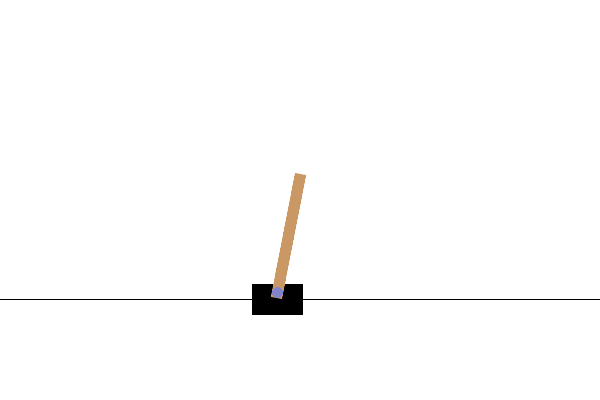
\includegraphics[width=0.5\textwidth]{Figures/cart_pole.png}
	\caption{The Cartpole environment.}
\end{figure}
The Cartpole environment is the "Hello World" of reinforcement learning; it describes a game where at each timestep, the aim is to balance a mass above a slider, 1 point is given for each timestep that the mass makes an angle of fewer than 12 degrees from vertical. The action space$a \in {0,1}$, for the problem, is to either push the pole left or right. The state space is the position of the cart, the velocity of the cart, the angle of the pole and the angular velocity of the pole; as such, $s \in \mathbb{R}^4$. Typically, the episodes are truncated at 500 timesteps, and the reward is 1, so the return is an integer $G_0 \in [0, 500]$. An episode terminates if the pole falls over or the cart moves too far from the centre. If a human were learning to solve this problem, one would notice that the expected result of pushing the cart left when it is leaning right at some positions is the same as pushing the cart right when it is leaning left at the displacement in the opposite direction. This is an example of symmetry in the problem, and it is this symmetry that we will attempt to exploit to improve the learning characteristics of the agent.

The symmetry present in Cartpole is the cyclic $C_2$ group. Other than the trivial group, the group with a single element, the $C_2$ group, is the simplest. This is a group with only two elements, the identity and inversion.
\begin{table}[h!]
	\centering
	\begin{tabular}{c | c  c}
		$C_2$ & $e$ & $r$ \\
		\hline
		$e$   & $e$ & $r$ \\
		$r$   & $r$ & $e$
	\end{tabular}
	\caption{The $C_2$ group table, where entry $i, j$ is the result of group operation on the $i^{th}$ and $j^{th}$ element.}
\end{table}


As such, to find the group structured MDP homomorphism, the agent needs to learn an equivariant mapping that respects $\pi_1^s\mathbf{s} = \mathbf{s}$ and $\pi_r^s\mathbf{s} = -\mathbf{s}$, as well as $\pi_1^a\mathbf{a} = \mathbf{a}$ and $\pi_r^a\mathbf{a} = 1 - \mathbf{a}$. Here the state and actions as vectors; $\mathbf{s}, \mathbf{a}$ are being acted upon by the vector representations of $C_2, \pi$ in their respective spaces.


\section{Neural Networks and The Inductive Biases}

What is nice in many ways about the original MLP model is that it is so flexible, however this also highlights one of its weaknesses when solving applied problems, because in theory MLPs have incredible expressive power, they are perfectly able to represent impossible functions, when applied to domains such as Images, and physical processes where there are concrete rules governing the processes that are being modelled\footnote{See the last few hundred years of Physics for examples.}. Additionally it is posited by~\cite{wolpert1995no}, that there is no free lunch in machine learning, and that there must be a constrained search space for possible algorithms. Such Constraints are in other words, inductive biases~\cite{baxter2000model}. This kind of reasoning has lead to much research into encoding inductive biases into Deep Networks, from~\cite{goyal2022inductive} a table of current approaches to introduce inductive biases;

\begin{table}
	\centering
\begin{tabular}{|c | c|}
	\hline
	Inductive Bias              & Corresponding property                              \\
	\hline
	\hline
	Distributed representations & Inputs mapped to patterns of features               \\
	\hline
	Convolution                 & group equivariance (usually over space)             \\
	\hline
	Deep architectures          & Complicated functions = composition of simpler ones \\
	\hline
	Graph Neural Networks       & equivariance over entities and relations            \\
	\hline
	Recurrent Nets              & equivariance over time                              \\
	\hline
	Soft attention              & equivariance over permutations                      \\
	\hline
	Self-supervised             & pre-training $P(X)$ is informative about $P(Y |X)$      \\
	\hline
\end{tabular}
\end{table}

For the purposes of this thesis, the focus will be on the induction of group eqivariances. However, it is important to note that this strategy to improving Machine Learning models comes from a more general class of ideas.


\subsection{Neural Networks and The Raiders of the Group}
\subsection{G-CNNs}\label{sec:G-CNNs}

The Group Equivariant Convolutional Neural Network (G-CNN) is a generalisation of the CNN's translational equivariance to arbitrary group structured equivariances.

The traditional Convolution layer is a discrete convolution, this is an approximation of tha continuous convolution,
\begin{equation}
	(f*g)(x) = \int_{\mathbb{R}^d} k(x-x')f(x')dy,
\end{equation}
where $f$ and $k$ are functions on $\mathbb{R}^d$. What can be noticed is that this is infact the definition of the cross correlaion between $f$ and $\ell_g[k]:  \mathbb{R}^d  \rightarrow \mathbb{R}^d$, where $\ell_g[k]$
is the translation group $\mathbb{R}^d$ acting on the kernel $k$,
\begin{align}
	(f*g)(x) & = \int_{\mathbb{R}^d} k(x-x')f(x')dx'       \\
	         & = \int_{\mathbb{R}^d} k(g^{-1}x')f(x')dx'   \\
	         & = \int_{\mathbb{R}^d} \ell_g[k](x')f(x')dx'
\end{align}
Here, the inverse of a tranlastion by $x$, group action $g$ is the translation by $-x$. This is then $g^{-1}$, the inverse of the group action. This is the backbone of the G-CNN\cite{cohen2016group}, where rather than a translation group, we have an arbitrary group $G$ acting on the kernel $k$. When looking for more complex equivariances than $C_2$, multiple different groups can be used in the same layer, this increases the number of varibles in the convolution's output, this complecates the form of the layers, however for our purposes this is not relevant.


\subsection{Steerabel Kernel G-CNNs}
% TODO: Add a section on Steerable Kernel G-CNNs
\chapter{Literature Review}\label{chap:litreview}

\section{Deep Learning and MDP Homomorphisms}
As discussed previously In Chapter \ref{chap:background} the idea of learning a Group Structured MDP homomorphism is a powerfull tool to make the learning problem posed by an MDP simpler. In this section I will discuss multiple parpers that attempt to learn Group Structured MDP Homomorphisms.
\subsection{MDP Homomorphic Networks}
\cite{vanderpol2020mdp} introduces the idea of performing policy based learning that respects the symmetry of the environment, by constraining the possible policies that can be represented by a neural network.

This is achieved by using an equivariant network on discrete action spaces. When the input to the network is transformed by a group structured operation, the output policy is also transformed by this operation, due to the equivariance property, and as such the network finds a more efficient method of learning the policy as the MDP problem it is solving is simpler, as it exploits the Group Structured MDP Homomorphism.

The equivariance in the deep network uses many of the same ideas as that of the G-CNNs\cite{cohen2016group}. In that the only requirement for a network to be equivaraint to a discrete group action's is that the individual layers of the network are equivariant to the group's actions. Despite the similarity, thier method of achieving the equivariance is quite different. The Authors propose the "symmetrizer layer". In contrast to the group convolution formulation, the symmetrizer layer achives equivaraince by finding weight matricies that are solutions to,
\begin{equation}
	\label{eqn:symmetrizer}
	\mat{W} =S(\mat{W}) = \frac{1}{|G|}\sum_{g\in G}{\pi_g^{\mathcal{X}'}}^{-1}\mat{W}\pi_g^{\mathcal{X}}
\end{equation}
Where if $f(\vec{x}) = \mat{W}\vec{x}$, $f: \mathcal{X} \rightarrow {\mathcal{X}'}$ and $\pi_g^{\mathcal{X}}$ is the representation of $g$ in $\mathcal{X}$, then $\pi_g^{\mathcal{X}'}$ is the representation of $g$ in $\mathcal{X}'$. In order to find such linear systems of equations in a general manner for a group $G$, the authors sample many matricies randomly from the space of all possible matricies of that size $\mathcal{W}_{total}$.Then apply the symmetrizer operation, $S$, to all of the sampled matricies.


From this point, because the symmetrizer operation is linear there exists a set of solutions to that linear equation,$\mathcal{W}$, and to form solutions to it, they vectorise and stack the found matricies, This forms a new matrix, which the singular value decomposition's basis vectors are orthogonal vectors of the equivariant subspace! These vectors $\{\mat{V}_i\}$ are all solutions to the above equation\ref{eqn:symmetrizer}. As such any linear combination of them is also a solution. Using the first $r$ vectors of the SVD, where $r= \text{rank}(\mathcal{W})$. An equivariant layer can by formed by,

\begin{equation}
	\mat{W} = \sum_{i=1}^{r}{\alpha_i\mat{V}_i}
\end{equation}

These layers have interesting properties in that the size of the subspace defines how many parameters when using this framework, there is no current closed form solution to the question of how many parameters each layer will have.

This scheme of producing equivariant layers, has some notable upsides, in that you only need to know how to trasform the input and output of the layer, $\mat{W} \rightarrow \mat{W}\pi_g^\mathcal{X}$ and $\mat{W} \rightarrow {\pi_g^{\mathcal{X}'}}^{-1} \mat{W}$ respectively. However, the scheme does require, expensive SVD calculations, in addition to the sampling of many matricies, which is expensive, but this only need be done once at the start of training per layer. However, there is no closed form solution to how many parameters the matricies will have, and as such the number of parameters in the network is not known until the SVD is performed.

The larger problems with this approach are that the homomorphisms must be exact, and known apriori. This limits the possible scenarios in which this approach can be used, as it is not always possible to know the exact symmetry. In addtion, to this in many cases generalising to continuous actions spaces is not possible with the current methodology.


\subsection{Group Equivariant Deep Reinforcement Leanrning}
In much the same vein as that of \cite{vanderpol2020mdp}, \cite{mondal2020group} proposes a method of exploiting equivariant networks for Deep RL, in comparison to \cite{vanderpol2020mdp}, they propose using G-CNNs\cite{cohen2016group} to achieve equivariance, rather than the symmetrizer layer. In contrast to leaning a policy they have a newtwork structure such that the states are mapped to an equivariant Latent space of dimension 256, This results in a network architure that can be thought of as an equivariant embedding function, $f(s)$, and a Q-Value function, $Q(s_{eqv}, a)$, acting on this space.
\begin{align}
	f: & \mathcal{S} \rightarrow \mathcal{S}_{eqv}      \\
	Q: & \mathcal{S}_{eqv} \rightarrow \mathbb{R}^{|A|}
\end{align}

One of the key downsides of this is it doesn't exploit the homomorphism of the MDP, that exists also in the action space. Despite this \cite{mondal2020group} still demonstrate an improvement in sample efficiency over a baselines of DDQN~\cite{van2016deep} and DQN~\cite{mnih2013playing} in snake. However, they onlt see a minor improvement in sample efficiency in Pacman, which also posseses the same $C_4$ group symmetry.

\subsection{$\mathrm{SO}(2)$ Equivariant Reinforcement Learning}

In much the same way as the above methods,~\cite{wang2022so2} also exploit exploit the equivariance property, in the context of robotic control in the PyBullet suite\cite{coumans2021}. They use steerable G-CNNs\cite{weiler2019general}, which provide $\text{SE}(2)$ equivariance, in robotic control environments. In contrast to previous papers where finite groups were exploited, the continuous Lie group $\text{SO}2$ constrains the degrees of freedom of the problem much more than the finite groups. Utilising this they are able to achieve impressive improvements in sample efficiency and robustness over conventional DQN and SAC mtehods.

In their first experiments of Drawer-Opening, Block Pulling, and Object Picking, the equivariant networks outperform all other DQN methods, and when applied to the SAC forumlation, In Objedct picking and Drawer Opening, they are the only methods that are able to solve the task.

Further they perform tests on more difficult robotic control tasks where demonstrations are provided, this enables the the agents to tackle more complex tasks such as block stacking and house building, in which they again are the only agents that are able to solve the tasks.

\section{Learning Models}

\chapter{Experiments}
\section{Environments}
Before diving into the experiments, the symmetric environments used are outlined below. Additionally, for notational convince the policy $\pi(a|s)$ is denoted as $\pi(s)$.
\section{CartPole}\label{sec:cartpole}
\begin{figure}[h!]
	\centering
	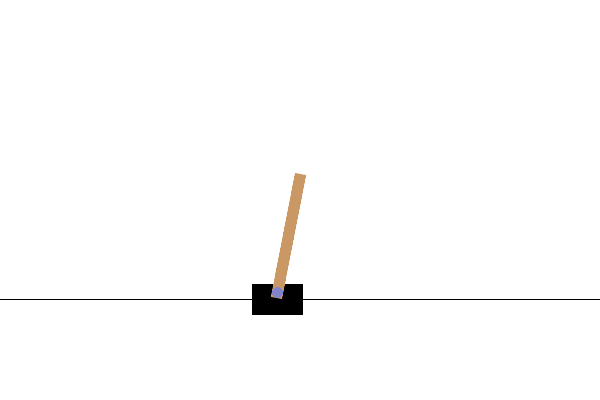
\includegraphics[width=0.5\textwidth]{Figures/cart_pole.png}
	\caption{The CartPole environment.}
\end{figure}
The CartPole environment is the "Hello World" of reinforcement learning; it describes a game where at each timestep, the aim is to balance a mass above a slider, 1 point is given for each timestep that the mass makes an angle of fewer than 12 degrees from vertical, in this instantiation. The action space$a \in {0,1}$ indicates pushing the pole left or right. The state space is the position of the cart, the velocity of the cart, the angle of the pole and the angular velocity of the pole. Then a state is a vector s:
\begin{equation}
	s = \begin{pmatrix}
		x       \\
		\dot{x} \\
		\theta  \\
		\dot{\theta}.
	\end{pmatrix}
\end{equation}
Thus, $s \in \mathbb{R}^4$.

Typically, the episodes are truncated at 500 timesteps, and the reward is 1, so the return is an integer $G_0 \in [0, 500]$. An episode terminates if the pole falls over or the cart moves too far from the centre. If a human were learning to solve this problem, one would notice that the expected result of pushing the cart left when it is leaning right at some positions is the same as pushing the cart right when it is leaning left at the displacement in the opposite direction. This is an example of symmetry in the problem, and it is this symmetry that is exploited by~\cite{vanderpol2020mdp, mondal2020group}.

To learn the transition dynamics of CartPole and agent must learn how the system evolves through time. In CartPole the transitions between different states in CartPole are governed by the PDEs:

\begin{equation}
	\ddot{\theta} = \frac{g \sin \theta + \cos\theta \left({\frac{-F - m_p l \dot{\theta}^2 \sin(\theta)}{m_c + m_p}} \right )}{l\left ( \frac{4}{3} - \frac{m_p \cos^2 \theta}{m_c + m_p}\right)},
\end{equation}

\begin{equation}
	\ddot{x} = \frac{ F + m_p l (\dot{\theta}^2 \sin \theta - \ddot{\theta} \cos \theta)}{m_c + m_p}.
\end{equation}
Here $g$ is the acceleration due to gravity and is positive, $\theta$ is the angle between the pole and vertical, with the pole length $l$. $F$ is the action force, where the positive direction is right. The masses of the cart and the pole are $m_c, m_p$, respectively. Finally, $\dot{}$, indicates a derivative with respect to time.

These PDEs have no closed solution and their form is taken from \cite{florian2007correct} who provides slight corrections to the original dynamics in \cite{barto1983neuronlike}.

Both learning a policy and a transition model may be augmented by exploiting symmetry. The symmetry present in CartPole is the cyclic $C_2$ group. Other than the trivial group, the group with a single element, the $C_2$ group, is the simplest. This is a group with only two elements, the identity and inversion.
\begin{table}[h]
	\begin{center}
		\begin{tabular}{c | c  c}
			$C_2$ & $e$ & $r$ \\
			\hline
			$e$   & $e$ & $r$ \\
			$r$   & $r$ & $e$ \\
		\end{tabular}
		\caption{The $C_2$ group table, where entry $i, j$ is the result of group operation on the $i^{th}$ and $j^{th}$ element.}
		\label{tab:cyclic_two}
	\end{center}
\end{table}


%%As such, to find the group structured MDP homomorphism, the agent needs to learn an equivariant mapping that respects $\pi_1^s\mathbf{s} = \mathbf{s}$ and $\pi_r^s\mathbf{s} = -\mathbf{s}$, as well as $\pi_1^a\mathbf{a} = \mathbf{a}$ and $\pi_r^a\mathbf{a} = 1 - \mathbf{a}$. Here the state and actions as vectors; $\mathbf{s}, \mathbf{a}$ are being acted upon by the vector representations of $C_2, \pi$ in their respective spaces.

\section{Catch}\label{sec:catch}
\begin{figure}[h!]
	\centering
	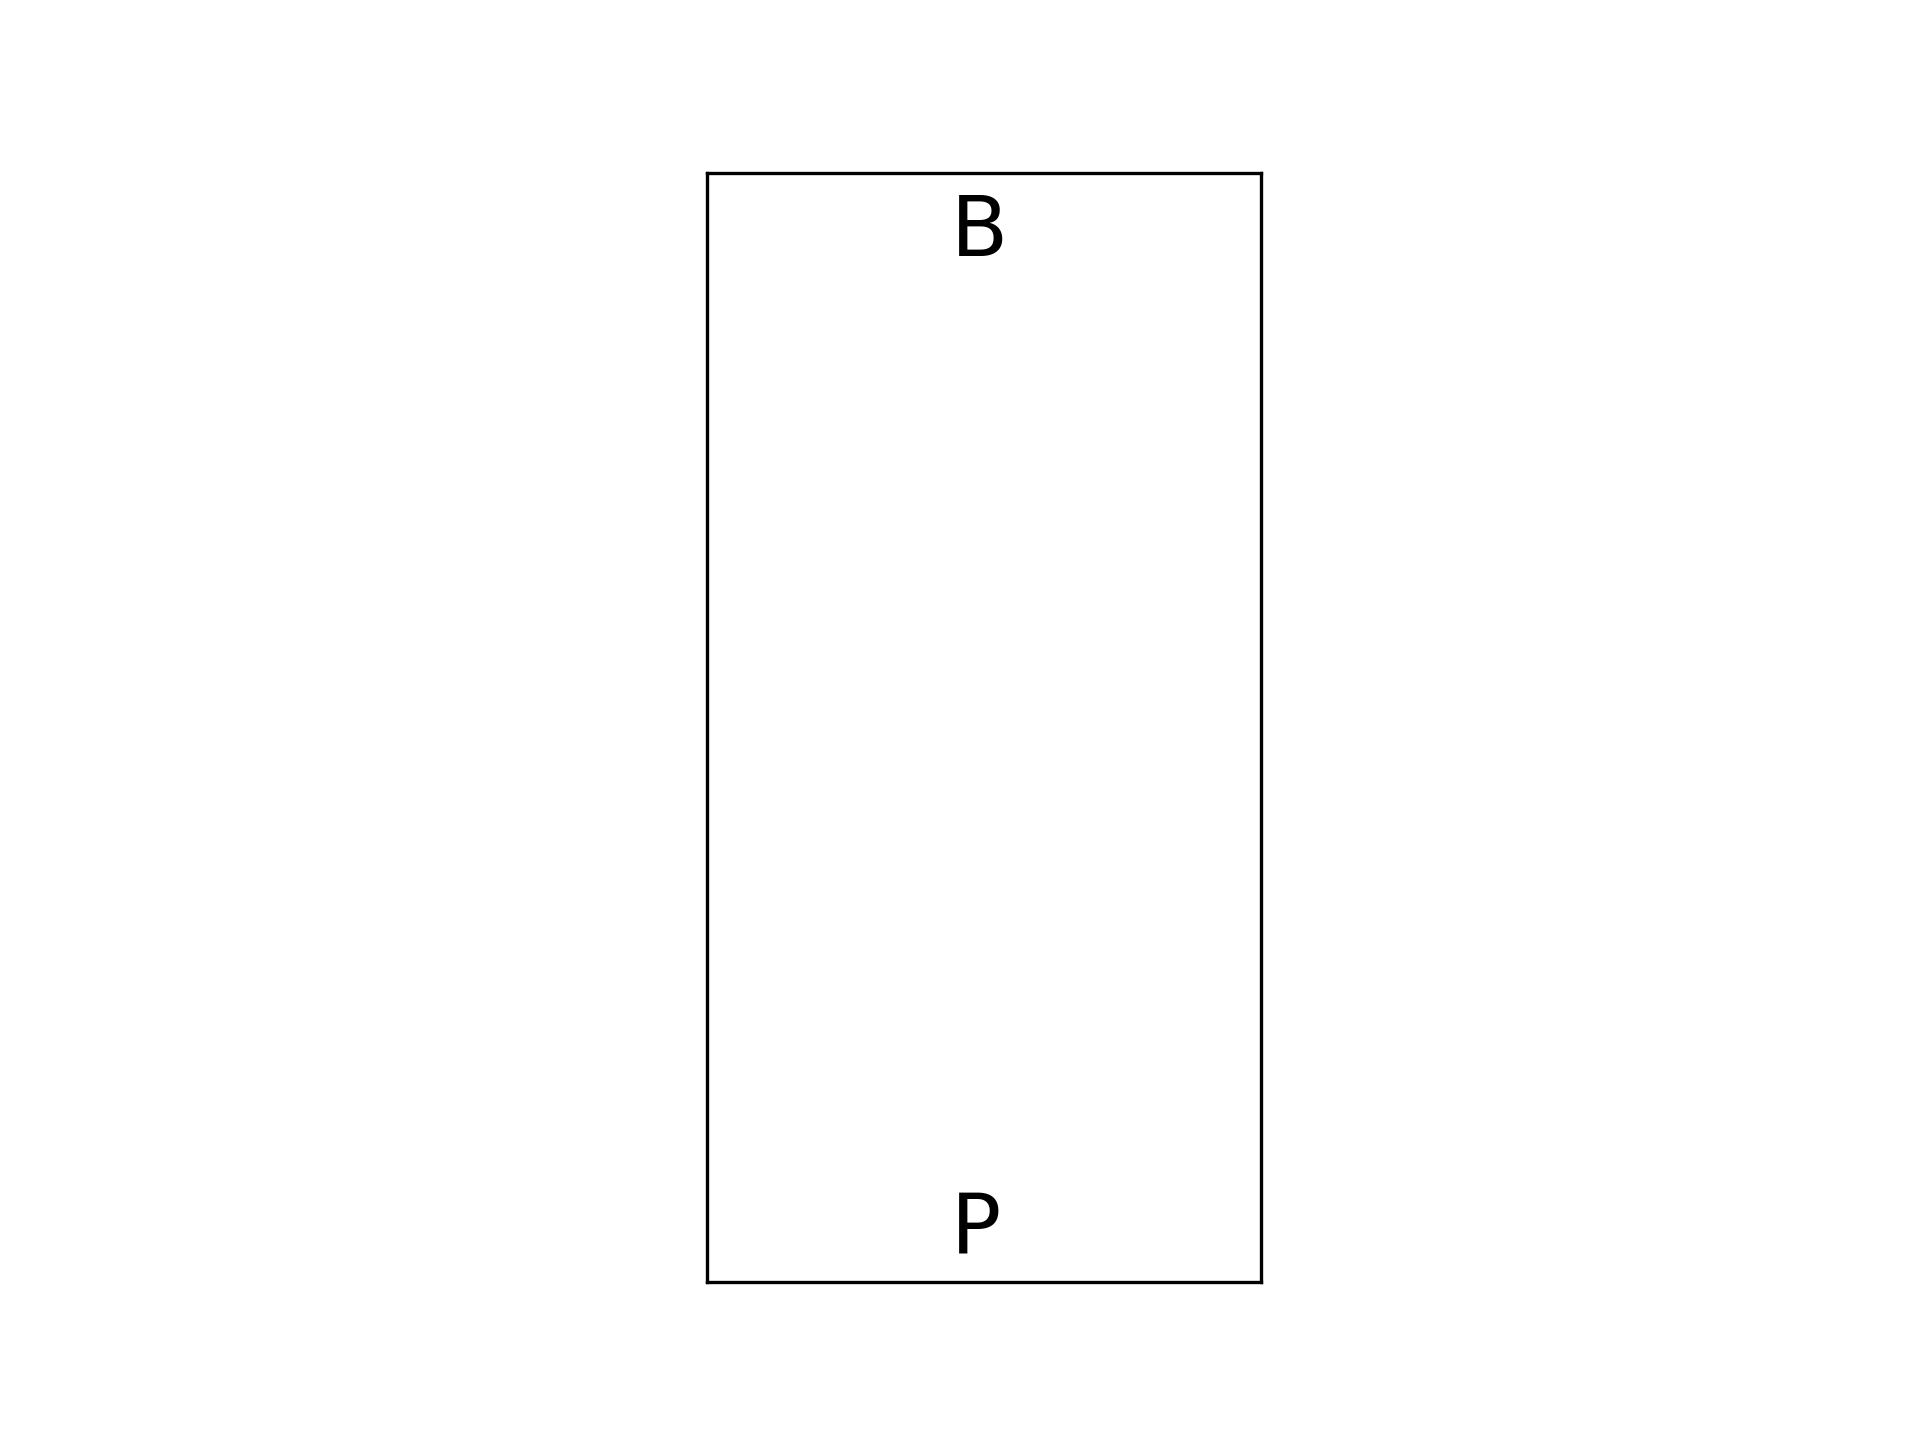
\includegraphics[width = 0.6\textwidth]{Figures/catch_env.png}
	\caption{The Catch environment. The ball position is indicated by B, and the paddle position is indicated by P.}
	\label{fig:catch_env}
\end{figure}
The Catch environment~\cite{osband2020bsuite} is another simple MDP task similar to CartPole used mainly for debugging implementations. The aim of the game is to catch a falling ball. The default implementation has ten rows and five columns. The ball moves down by one row every time-step, and the position of the paddle is translated left or right by the action of the agent. When the ball reaches the tenth row, the reward of the system is $+1$, if the ball and the paddle are in the same location, otherwise the reward is $-1$. For all other time-steps the reward is zero. This produces an episodic environment, with a maximum return of one.

The state and action spaces are both discrete, and the transitions are deterministic. These states are represented to the agent as a $5\times 10$ array, with the ball and paddle's positions indicated by ones. The actions the agent can take are $\mathcal{A} = [0, 1, 2]$, that translate the ball by $1-a$. Thus, the MDP has a finite amount of transitions and state action pairs, 675 in total.

Like CartPole, the Catch environment possesses $C_2$ group symmetry, however, due to the different state and action spaces the representations of the groups are different. However, because the groups are the same the structure is that in Table.\ref{tab:cyclic_two}.

\section{Motivation}
A series of Experiments were carried out to investigate the efficacy of equivariant transition model structure in model-based RL problems with symmetric environments. Where the specific model-based algorithm investigated was Dyna.

Model-based RL, is inherently more complex than actor-critic or value based methods, as not only does a policy need to be learned, but also a model of the environment dynamics must also be learned. In the case of a NN model, this will require training a model, as well as an agent.

Even with the simple models constructed here, the model based agents have two times more parameters. Within wider literature, models such as Dreamer-v3~\cite{hafner2023mastering}, use 8 million parameters, and multiple GPU days to learn policies on the complete Bsuite~\cite{osband2020bsuite} environment.

The increased complexity in the Dyna algorithm is mitigated by its modularity. The Dyna agent is constructed out of a transition model and a model-free agent. This provides a sensible progression for development and experimentation. Firstly, the model-free agent was constructed, and the symmetric inductive biase was tested only for the agent. Then, transition models were trained offline and tested. Finally these disjoint pieces were brought together to form the full Dyna implementation.

\section{Baseline}\label{sec:baseline}
The baseline that was chosen was a proximal policy optimization, Sec.\ref{sec:PPO}, agent from PureJaxRL,~\cite{lu2022discovered, schulman2015highdimensional}. This baseline provides a training framework, that trains a single agent concurrently on multiple identical environments. The training regime is outlined below in pseudocode.
\begin{algorithm}
	\caption{PureJaxRL PPO Agent Training Structure}
	\begin{algorithmic}
		\State Initialize agent: actor-critic $\pi_\theta$, $v_\phi$
		\State Initialize replay buffer: $\mathcal{D}$
		\For{Num Updates}
		\State Gain experience for Num Timestep
		\State Store trajectories: $\mathcal{D}$.append($(S, A, S', R))$
		\State Calculate GAE estimate from experience timesteps
		\For{ Num Epochs}
		\State{ Split GAE estimates into minibatches}
		\State{ Mini-Batch SGD with Adam on $\pi_\theta, v_\phi$}
		\Comment{ See~\ref{sec:PPO} for losses to optimize}
		\EndFor
		\EndFor
		\State Returns($\mathcal{D}$)

	\end{algorithmic}
\end{algorithm}

\section{Equivariant Actor-Critics}\label{sec:actor-critic}
\subsection{CartPole}

To form an equivariant network to the group structure of CartPole the actor network must be equivariant to both the identity and inversion operator. This report provides structures for equivariant G-CNNs for both CartPole and Catch, that can easily be extended to other environments with known discrete symmetries.

\subsubsection{Constructing a CartPole Actor-Critic}
In this section, the outline for the network design is described. In the Catch section, Sec.\ref{sec:catch_ac}, a more detailed description of how to extend the procedure to other groups is outlined.
The group for CartPole contains two unique elements, in both state and action space. In state space the inversion and identity operator $e, r$ are,
\begin{equation}
	\ell^\mathcal{S}_e =
	\begin{pmatrix}
		1 & 0 & 0 & 0 \\
		0 & 1 & 0 & 0 \\
		0 & 0 & 1 & 0 \\
		0 & 0 & 0 & 1 \\
	\end{pmatrix},
	\ell^\mathcal{S}_r =
	\begin{pmatrix}
		-1 & 0  & 0  & 0  \\
		0  & -1 & 0  & 0  \\
		0  & 0  & -1 & 0  \\
		0  & 0  & 0  & -1 \\
	\end{pmatrix}.
\end{equation}
Then the action space, the inversion and identity operator are,
\begin{equation}
	\ell^\mathcal{A}_e =
	\begin{pmatrix}
		1 & 0 \\
		0 & 1 \\
	\end{pmatrix},
	\ell^\mathcal{A}_r =
	\begin{pmatrix}
		0 & 1 \\
		1 & 0 \\
	\end{pmatrix}.
\end{equation}
Thus, to parametrize an equivariant actor network, the network $\pi_\theta$ must satisfy,
\begin{equation}
	\pi_\theta(\ell^\mathcal{S}_e s) = \ell^\mathcal{A}_e \pi_\theta(s),
\end{equation}
\begin{equation}
	\pi_\theta(\ell^\mathcal{S}_r s) = \ell^\mathcal{A}_r \pi_\theta(s).
\end{equation}
Instead of using a G-CNN for the Actor-Critic, a simpler solution involves employing a network with only odd operations, such as the tanh activation, and excluding biases for all hidden representations. By definition, odd functions are equivariant to both inversion and identity transformations, ensuring the network's equivariance. However, this doesn't address the issue of equivariance in the action space. To bridge this gap, a group convolution layer is incorporated to map between representations.

The network can be considered as a composition of $f_\theta : \mathcal{S} \rightarrow \mathbb{R}^{|H|}$, an odd embedding MLP and $gc_\theta: \mathbb{R}^{|H|} \rightarrow \mathbb{R}^{\mathcal{A}}$ a group convolution layer that ``lifts" the equivariance to the action space. As such the parametric policy is,
\begin{equation}
	\pi_\theta(s) = gc_\theta(f_\theta(s)).
\end{equation}
The equivariance properties of the sub-networks with respect to the inversion operator are,
\begin{equation}
	f_\theta(-s) = -f_\theta(s),
\end{equation}
\begin{equation}
	gc_\theta(-x) =
	\begin{pmatrix}
		0 & 1 \\
		1 & 0 \\
	\end{pmatrix}
	gc_\theta(x),
\end{equation}
Where $gc_\theta(x) = [P(A=a_0), P(A=a_1)]$ describes the distribution over the binary actions of CartPole.

This G-CNN network for policy learning is the first novel contribution of this report. In comparison to the work of \cite{mondal2020group}, the policy learning G-CNN is fully equivariant, rather than learning action values from an equivariant embedding. Additionally, the network parametrizes a policy directly rather than Q values. Due to the network's end to end equivariance in comparison to the Q-value network proposed by \cite{mondal2020group}, agents parametrized by this network must take the same actions in states that are in the same orbit, which is not the case for the Q-value network, which only has an equivariant embedding. Thus, they do not guarantee equivariance in the policy.

Further, this network architecture has advantages over Symmetrizer networks, \cite{vanderpol2020mdp}, in that it does not require a large matrix inversions to solve for the parameters of the network, while still maintaining the same equivariance qualities.

\subsubsection{Results: Training Dynamics On the CartPole Benchmark}
With the network's structure established, the benchmark task focuses on mastering an expert policy within the CartPole environment. By default, CartPole imposes a maximum episode length of 500 interactions. All non-terminal states yield a reward of +1, setting the maximum episodic return at 500. As with most traditional RL problems, the primary objective in CartPole is to optimize the agent's episodic return. Finding an expert policy in CartPole using standard deep learning methods is relatively straightforward and primarily serves as an implementation benchmark. For an equivariant network structure to truly enhance the quality of the learned policy, it should strive to approach the 500 episodic return benchmark with fewer environment interactions.

When comparing the learning dynamics of policy agents, it's crucial to ensure not just that the agent achieves expertise in the task but also that the policy learning procedure remains stable across multiple random seeds. A random seed refers to the initial state in which both the agent and environment begin. Keeping training stability in mind, examining the performance under the least favourable random seeds is informative about the training robustness. If an algorithm is particularly sensitive to its initialization, its performance may be significantly impacted, and may not converge over multiple random seeds~\cite{henderson2018deep}.

For all experiments, we utilize a standard MLP for the critic without imposing any equivariance constraints. While this setup might not yield optimal performance, it's essential to highlight that training is conducted across 128 random seeds to ensure the stability of the agent's learning.

Due to constraints on the equivariant network structures, it's not always feasible to maintain an identical number of parameters across networks. In instances where the exact parameter count differs, we ensure that the depth of all networks remains constant. We then adjust the width to achieve a parameter count that's within 10\% of the MLP baseline.

Refer to Fig.\ref{fig:cp_equi_ac} below, where the mean episodic return of three agents with distinct network architectures is illustrated. Despite the differences in their structures, all networks share the same training hyperparameters, as provided in the PureJaxRL\cite{lu2022discovered} baselines. The three networks depicted are the MLP baseline from PureJaxRL, an implementation of the Symmetrizer network from \cite{vanderpol2020mdp}, and the G-CNN policy network introduced in this report.

\begin{figure}[h!]
	\begin{center}
		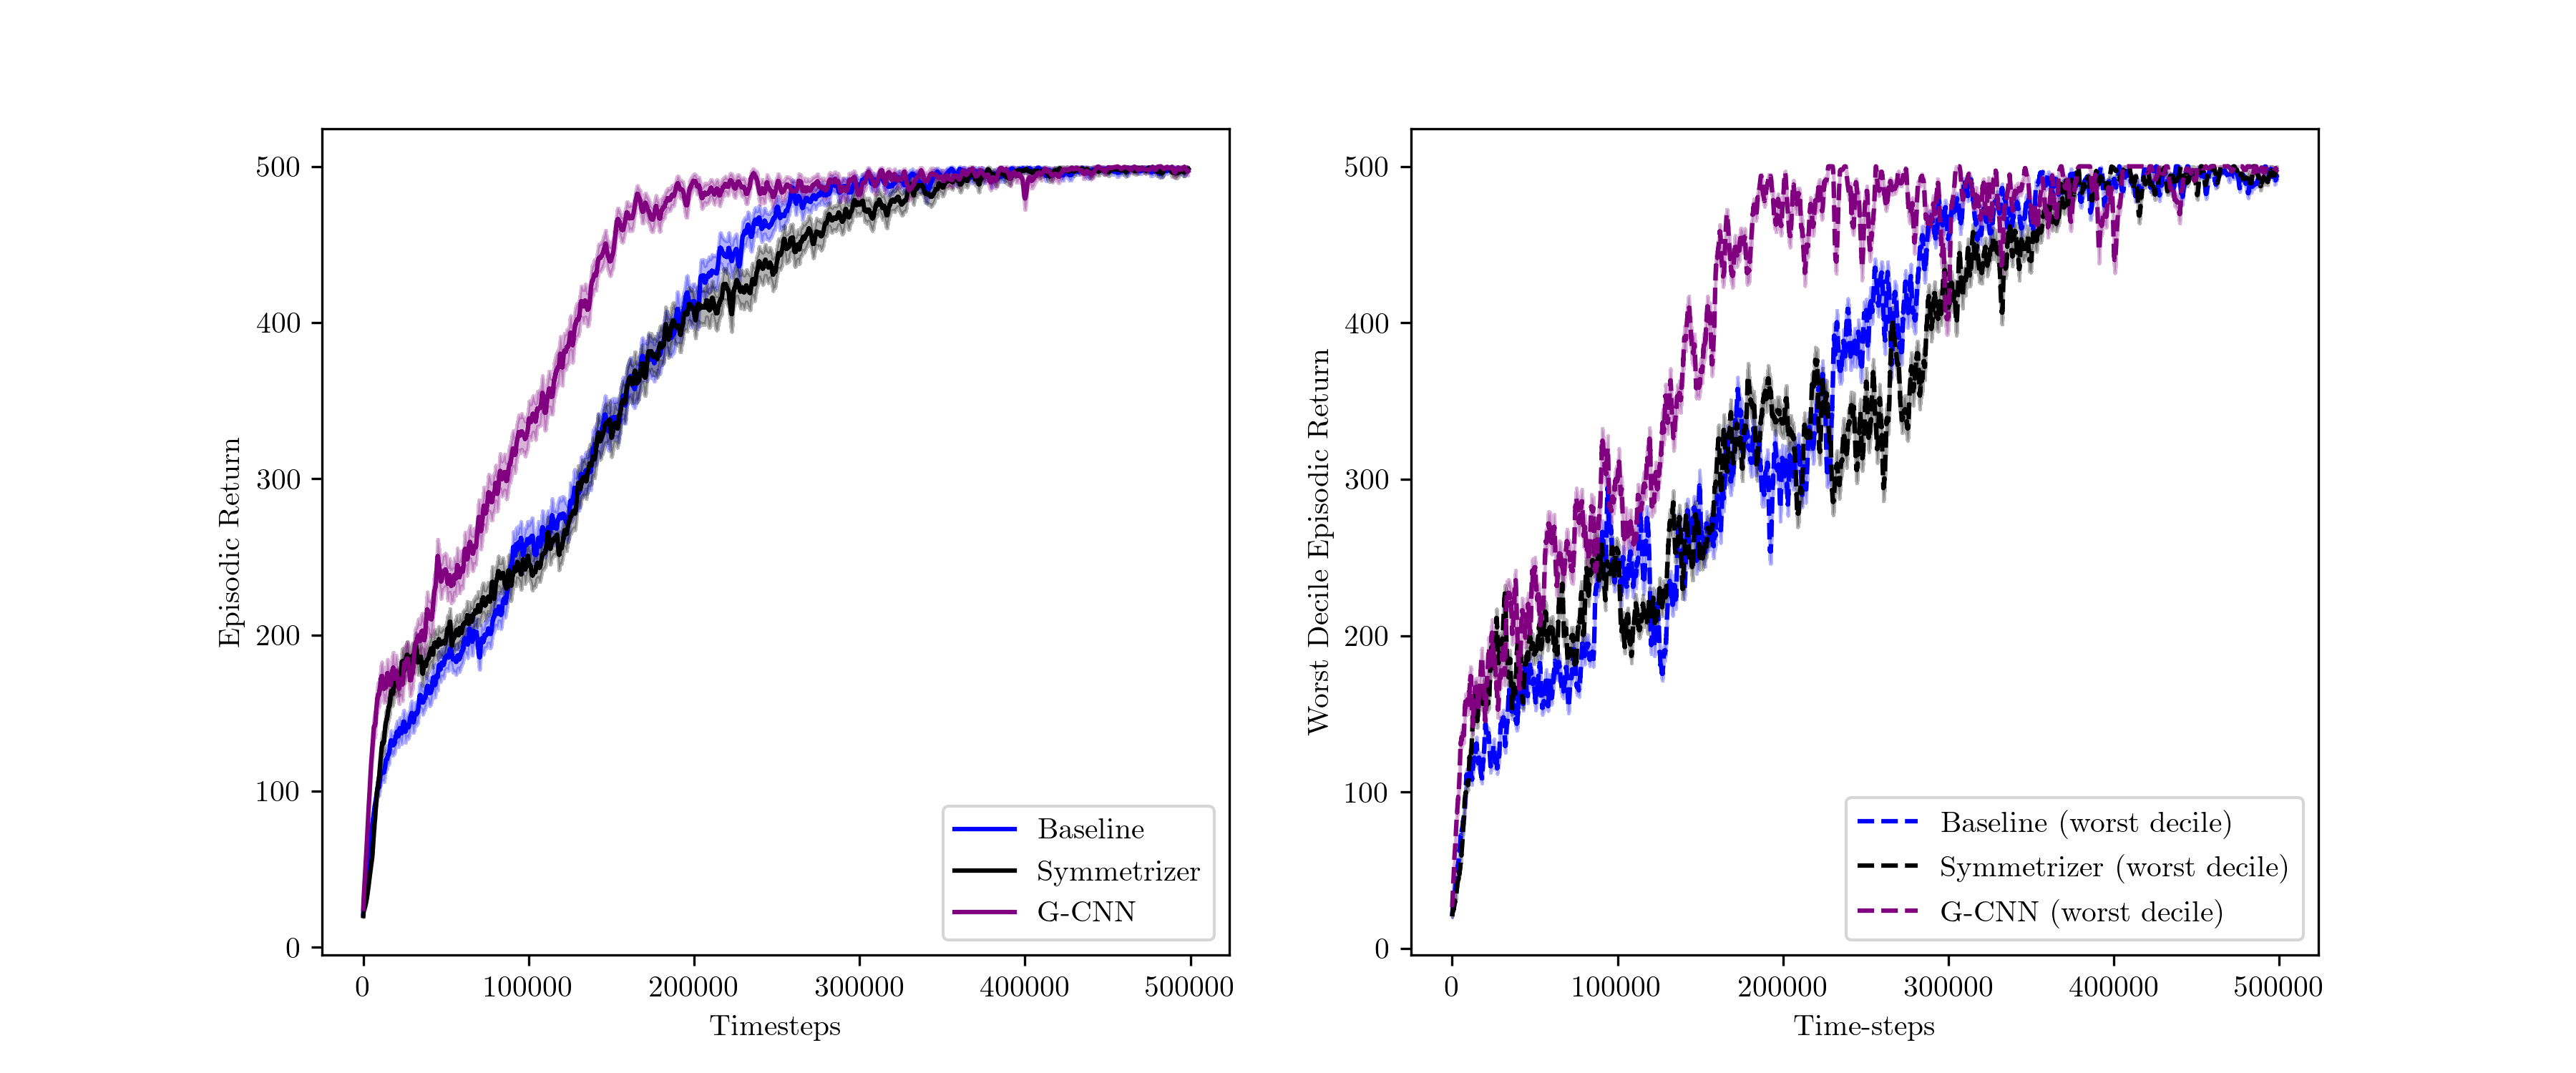
\includegraphics[width=\linewidth]{Figures/cart_pole_returns.png}
		\caption{Left: Mean episodic returns for the CartPole agents across 128 random seeds plotted against number of experience time-steps in the MDP. Right: The mean cumulative episodic returns of the worst performing 128 random seeds against number of experience time-steps in the MDP. Both of the plots are moving averages, with windows of 10 time-steps. Additionally, all plots have two standard errors plotted. }
		\label{fig:cp_equi_ac}
	\end{center}
\end{figure}

Both the Symmetrizer and the G-CNN are equivariant to the actions of the $C_2$ group. This equivariance constraint requires a learned policy that respects the inversion symmetry present in CartPole. The equivariance  should improve the sample efficiency of the agent as any learning from one state additionally informs the agent about the agent about the policy for the other state in the orbit. This hypothesis, is supported somewhat by the observed training dynamics. Over the first period of training, both the Symmetrizer and the G-CNN, outperform the baseline. This is more clearly illustrated in Table.\ref{tab:actor-critic}, where the G-CNN actor-critic has a $54\%$ increase in return over the baseline at 10,000 timsteps. The Symmetrizer, does not maintain this performance advantage. Our implementation uses the same network size, as the original paper and the same network hyperparameters. Despite this, the Symmetrizer agent fails to learn an expert policy in fewer steps than that of the baseline.

It should be noted that here the mean plus minus two standard deviations is plotted in comparison to the median and upper and lower quartiles of cumulative returns, which is plotted in \cite{vanderpol2020mdp}. The performance of the Symmetrizer, is underwhelming despite the implemented network being checked for equivariance. Further tuning of the hyperparameters may yield performance that improves upon the baseline's returns. However, this was not a primary concern in this report.

The G-CNN does compare favourably with the baseline implementation of an MLP, having slightly fewer parameters. It can be seen that it both converges on average to an expert policy in fewer time-steps but also has a more favourable convergence behaviour in challenging initialization conditions. This can be seen in the right of Figure \ref{fig:cp_equi_ac} where, the bottom tenth percentile of cumulative returns, still converges notably faster than that of the baseline.

\begin{table}
	\centering
	\begin{tabular}{|c|c|c|c|}
		\hline
		Timesteps  & Baseline     & Symmetrizer          & G-CNN                 \\
		\hline
		$10, 000$  & $102 \pm 5$  & $116 \pm 6$          & $\mathbf{158 \pm 8}$  \\
		$100, 000$ & $260 \pm 10$ & $240 \pm$ 10         & $\mathbf{330 \pm 10}$ \\
		$500,000$  & $497 \pm 1$  & $\mathbf{500 \pm 1}$ & $499 \pm 1$           \\
		\hline
	\end{tabular}
	\caption{Mean episodic returns across 128 random seeds tabulated for the three network architectures at three timesteps. All episodic returns are recorded with confidence intervals of two standard errors across 128 random seeds.}
	\label{tab:actor-critic}
\end{table}
Additionally, the mean episodic returns across all random seeds are tabulated at $10,000$, $100,000$, and $500,000$ time-steps in Table \ref{tab:actor-critic}. Upon closer inspection, the G-CNN agent incorporating the equivariant inductive bias significantly outperforms the baseline at all tabulated timesteps.

While both models have similar parameter counts, the structure of the G-CNNs makes their forward passes more computationally intensive. This is due to the G-CNN architecture requiring twice as many operations in a forward pass, attributed to the two group actions. However, in a scenario like CartPole, where the networks are relatively small and inexpensive to evaluate—and where computation can be efficiently parallelized—both models can train 128 random seeds in under a minute. This speed is achieved using the hyperparameters listed in the Appendix and executed on a RTX 3090.

Encouraged by the promising results from the initial experiment, we decided to explore a new environment to determine whether the equivariance constraint could further enhance performance.

\subsection{Catch}\label{sec:catch_ac}
To demonstrate that G-CNN actor-critic can be extended to other environments with different group actions, we implemented the equivariant actor-critic for the Bsuite Catch environment~\cite{osband2020bsuite}. For the Catch environment, constructing an equivariant network is challenging.

\subsubsection{Constructing a Catch Actor-Critic}
Unlike the CartPole case where layers can be made equivariant to the
representation, in Catch, the entire network must be built using Group Convolutions. As in previous scenarios, we impose an equivariant constraint on the actor $\pi_\theta(s)$.
In the context of Catch, the input state space is represented as $\mathcal{S} \in [0, 1]^{50}$. Instead of detailing the cumbersome $\ell_r^\mathcal{S} \in \mathcal{R}^{50 \times 50}$ matrix representation of the reflection group action $\ell_r^\mathcal{S}$, it is left symbolically. This action modifies the x-coordinate of both the ball and the paddle using the transformation $r(x)=-(2-x)$. Thus, the equivariance constraint is expressed as:
\begin{equation}
	\pi_\theta(\ell_r^\mathcal{S} s) = \begin{pmatrix}
		0 & 0 & 1 \\
		0 & 1 & 0 \\
		1 & 0 & 0 \\
	\end{pmatrix}\pi_\theta(s).
\end{equation}
% To demonstrate that G-CNN actor-critics extend to other environments, with different group actions. The equivariant actor-critic is implemented for the Bsuite~\cite{osband2020bsuite} Catch environment. In the case of the Catch environment to make an equivariant network because layers themselves are not easily made equivariant to the C2 representation, like in the case of CartPole, the whole network must be constructed out of Group Convolutions. As before, we consider equivariant constraint on the actor $\pi_\theta(s)$.
%
% In the case of catch the input state space is $\mathcal{S} \in [0, 1]^{50}$. Avoiding writing out the tedious matrix representation of the reflection action $r$, it is left as $\ell_r^\mathcal{S}$. This action takes the x co-ordinate of the ball and the paddle and transforms them by, $r(x) = -(2-x)$. Thus, the equivariance constraint is,
% \begin{equation}
% 	\pi_\theta(\ell_r^\mathcal{S} s) = \begin{pmatrix}
% 		0 & 0 & 1 \\
% 		0 & 1 & 0 \\
% 		1 & 0 & 0
% 	\end{pmatrix}\pi_\theta(s).
% \end{equation}

To construct a G-CNN, which is equivariant to the group actions a group action in the hidden layers must be determined. Consider a group convolution input layer $f : \mathcal{S} \rightarrow \mathcal{H} \in \mathbb{R}^{|G| \times |H|}$, commonly referred to as a lifting layer that maps from a state space to a hidden space of $H$. Lifting layers apply a group action to the input and then passes the transformed input through, $ g: \mathcal{S} \rightarrow \mathbb{R}^{|H|}$, a dense/convolution layer. In the full layer the input is transformed by every group action, and then passed through $g$. In the absence of any pooling, this gives a hidden representation, that is the hidden dimensions of the equivalent dense/convolution layer, plus a new axis that is the size of the group. To illustrate the new equivariance constraint a single layer;
\begin{equation}
	g(s) = \vec{h} \in \mathbb{R}^{|H|}.
\end{equation}
When formed into a group convolution,
\begin{equation}
	f(s) = \begin{pmatrix}
		g(s)                   \\
		g(\ell_1^\mathcal{S}s) \\
		g(\ell^\mathcal{S}_2s) \\
		\vdots                 \\
		g(\ell_{|G|}s).
	\end{pmatrix}
\end{equation}
Once a group action is applied to the input, the output values undergo permutation. While the exact permutation is contingent on the group, the permutations' structure can be readily determined due to group closure:
% When a group action is applied to the input the values of the output are permuted. The exact permutation depends upon the group, however, the structure of the permutations are easily calculated due to group closure;
\begin{equation}\label{eq:gs_perm}
	f(\ell_n^\mathcal{S}s) = \begin{pmatrix}
		g(\ell_n^\mathcal{S}s)                   \\
		g(\ell_n^\mathcal{S}\ell_1^\mathcal{S}s) \\
		g(\ell_n^\mathcal{S}\ell_{|G|}s)         \\
		\vdots                                   \\
		g(\ell_n^\mathcal{S}\ell_{|G|}s)         \\
	\end{pmatrix}
	= \begin{pmatrix}
		g(\ell_n^\mathcal{S}s) \\
		g(\ell_i^\mathcal{S}s) \\
		g(\ell^\mathcal{S}_js) \\
		\vdots                 \\
		g(\ell_{k}s).
	\end{pmatrix}
	= \mat{P}_n f(s)
\end{equation}
Where $\mat{P}_n$, is a permutation matrix defined by the group. There is a unique permutation matrix for each group element. This permutation relation enables one to construct further equivariant layers. Consider a subsequent, $h: \mathcal{H} \rightarrow \mathcal{H}'$, a hidden layer that must continue the equivariance to group G. This is achieved by treating each $\mat{P}$ as the group action, and ensuring that the output is equivariant to its application. The new layer can be through of as taking a vector of responses, where it must be equivariant to the vectors' permutation,
\begin{equation}
	h\left( \mat{P_i}
	\begin{pmatrix}
		v_1    \\
		v_2    \\
		\vdots \\
		v_{|G|}
	\end{pmatrix}
	\right) = \mat{P_i} h
	\begin{pmatrix}
		v_1    \\
		v_2    \\
		\vdots \\
		v_{|G|}
	\end{pmatrix}.
\end{equation}
Tying this to a concrete example in a 1D convolution, if there is an input that is one hot, and the kernel has a single weight, $w_1$. The output of the layer will be;
\begin{equation}
	\text{Conv1D}\begin{pmatrix}
		0 \\
		1 \\
		0 \\
	\end{pmatrix}
	= \begin{pmatrix}
		0   \\
		w_1 \\
		0   \\
	\end{pmatrix}
\end{equation}
If the input is translated the output is also translated;
\begin{equation}
	\text{Conv1D}\begin{pmatrix}
		1 \\
		0 \\
		0 \\
	\end{pmatrix}
	= \begin{pmatrix}
		w_1 \\
		0   \\
		0   \\
	\end{pmatrix}
\end{equation}
Which is the definition of the equivariant constraint, slightly more abstractly\footnote{If you are slightly shocked by the order of the group actions acting on x here, dont be. It comes from the relationship between the right and left action on the kernel see~\cite{cohen2016group}};
\begin{equation}
	\text{Conv1D}(x) = \begin{pmatrix}
		g(\ell_{1}x)   \\
		g(x)           \\
		g(\ell_{-1} x) \\
	\end{pmatrix}
\end{equation}
Then when the input is translated up by one $\ell_{-1}$;
\begin{equation}\label{eq:perm_gr}
	\text{Conv1D}(\ell_{-1} x) = \begin{pmatrix}
		g(\ell_{1}\ell_{-1}x)   \\
		g(\ell_{-1}x)           \\
		g(\ell_{-1}\ell_{-1} x) \\
	\end{pmatrix}
\end{equation}
And the closure of the group defines its permutation. The group table for this translation group is given below.
\begin{table}[h]
	\centering
	\begin{tabular}{|c| c c c|}
		\hline
		G  & -1 & 0  & 1  \\
		\hline
		-1 & 1  & -1 & 0  \\
		0  & -1 & 0  & 1  \\
		1  & 0  & 1  & -1 \\
		\hline
	\end{tabular}
	\caption{Example translation group.}
\end{table}
By using this Eq.\ref{eq:perm_gr} becomes;

\begin{equation}
	\text{Conv1D}(\ell_{-1} x) = \begin{pmatrix}
		g(x)          \\
		g(\ell_{-1}x) \\
		g(\ell_{1}x)  \\
	\end{pmatrix}
\end{equation}
Which is a permutation of the input governed by the group structure of Eq.\ref{eq:gs_perm}.

Given this equivariant structure for each layer, when constructing a network out of an input layer and subsequent hidden layers that all adhere to the equivariance constraint, what remains is to identify an appropriate output. In scenarios such as an actor network operating within a discrete action space, the permutation representation proves ideal. For instance, in the Catch environment, the probability of moving left in state \( s \) should mirror the probability of moving right in its reflected state \( s' = \ell_r^\mathcal{S} \). Since the network produces logits, un-normalized probabilities, their permutation upon reflection possesses the desired properties. However, when a permutation doesn't fit the necessary group action, establishing equivariance becomes more intricate. This challenge will be delved into in subsequent sections, Sec.\ref{sec:tm_catch}.

With the framework of an equivariant network in place, similar to the CartPole scenario. Both an equivariant actor-critic and an MLP actor-critic, were established. These were designed with two hidden layers and an approximate equivalent in parameter count. For this experiment, the Symmetrizer was omitted due to the difficulties encountered when trying to optimize its performance, as depicted in the primary study. Given the small state-action space of the Catch task relative to CartPole, agents were allotted 20,000 MDP interactions for learning. The MLP baseline once again employed the PureJaxRL baseline actor-critic, albeit with minor modifications for adaptation to the new environment. Both network architectures were assigned identical hyperparameters, Appendix.\ref{ap:hyp}.

\subsubsection{Results: Training Dynamics On the Catch Benchmark}
% With this equivariant structure for each layer the network constructed out of an input layer and subsequent hidden layers, which all maintain the equivariance constraint, the only thing left is to find an output. In the case of an actor network in a discrete action space, the permutation representation, is perfect, in the case of Catch where the probability of moving left in a state $s$ should be the same as the probability of moving right in a reflected state $s' = \ell_r^\mathcal{S}$. As the network outputs logits, un-normalised probabilities, their permutation on a reflection is the exact property required. For cases where a permutation is not the required group action, achieving equivariance is slightly more difficult. This is left for later.
%
% With an Equivariant network structure created, as in the case of CartPole, an Equivariant actor critic and an MLP actor critic were formed with two hidden layers, and a comparable parameter count. In this experiment, the Symmetrizer was left out due to the challenges found optimizing its performance to that demonstrated in the original paper. As Catch is a much more straightforward task, the agents are given $20,000$ MDP interactions to learn over in comparison to that of CartPole, again the MLP baseline is the PureJaxRL baseline actor-critic, slightly adjusted for the new environment. Both network architectures were given the same hyperparameters.

\begin{figure}
	\centering
	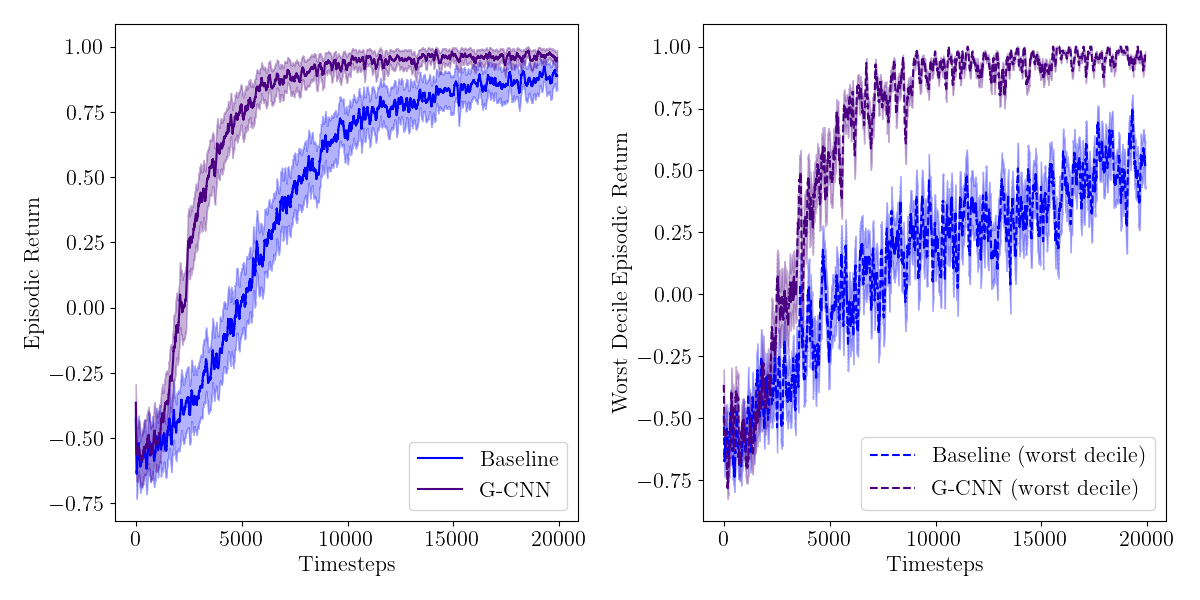
\includegraphics[width=\linewidth]{Figures/catch_returns.png}
	\caption{Left: Mean episodic returns for the Catch agents across 128 random seeds plotted against number of interaction time-steps in the MDP. Right: The mean cumulative episodic returns of the worst performing 128 random seeds against number of experience time-steps in the MDP. Both of the plots are moving averages, with windows of 10 time-steps. Additionally, two standard errors are plotted.}
\end{figure}
Upon examining the qualitative differences in the episodic return curves, we observe a familiar yet more pronounced trend. For Catch, the inductive bias of equivariance seems especially beneficial. Not only does the agent with the G-CNN converge to an expert policy more rapidly than its counterpart, but the bottom decile of random seeds also exhibits markedly improved performance. Furthermore, by referring to the tabulated results in Table~\ref{tab:actor-critic_catch}, the superiority of the Equivariant Network architecture is evident. It manages to achieve a higher proficiency in Catch in half the time, achieving a higher mean return at 10,000 timesteps than the baseline at 20,000 timesteps.

% Again, looking at the qualitative performance difference from the Episodic return curves we see a similar but more exaggerated story. For Catch the equivariance inductive bias appears to be incredibly useful, and not only does the agent converge to an expert policy faster, than without the G-CNN, but also the bottom decile of random seeds also perform substantially better. Further, looking at tabulated performance in Table~\ref{tab:actor-critic_catch}, The dominance of the Equivariant Network architecture is apparent, with it achieving a greater mastery of Catch in half of the time.

\begin{table}
	\centering
	\begin{tabular}{|c|c|c|}
		\hline
		Timesteps & Baseline         & G-CNN                     \\
		\hline
		$2, 000$  & $- 0.51\pm 0.07$ & $\mathbf{-0.06 \pm 0.09}$ \\
		$10, 000$ & $0.70 \pm 0.06$  & $\mathbf{0.95 \pm 0.03} $ \\
		$20,000$  & $0.875 \pm 0.04$ & $\mathbf{0.96\pm 0.02}$   \\
		\hline
	\end{tabular}
	\caption{Mean episodic returns across 128 random seeds tabulated for the two network architectures at three timesteps. All episodic returns are recorded with confidence intervals of two standard errors across 128 random seeds.}
	\label{tab:actor-critic_catch}
\end{table}
\subsection{Conclusion}
Equivariant actors were tested in both environments, and showed a substantially more efficient learning. These results are inline with other experiments, where agents are trained with inductive biases about the task's symmetry outperform conventional methods. Further, they also demonstrated the same improvement in cases with challenging initialization conditions.

The equivariance constraint itself however, is quite limiting. For any given task the group must be known beforehand. Not only this but it must also be an exact symmetry. In many settings these constraints are rare, especially with discrete symmetry groups.

Additionally, there is a forward pass cost to the equivariant network structure, especially with larger groups, despite the same number of parameters being used. With the way G-CNNs are constructed, the number of operations in a forward pass of the network is $\mathcal{O}(|G|)$. As such, the inference time increases when including the inductive bias. However, because these operations can be executed in parallel, the evaluation time increase is limited. For a rough estimation of the increased overhead the G-CNN. The implementations of the G-CNN for catch and the MLP were benchmarked. The MLP's mean forward pass over $10000$ states was $27.5 \pm 0.1\mu s$, and $29.9 \pm 0.1 \mu s$ for the G-CNN. This is an $8\%$ increase in evaluation time, with similar standard error across 1000 tests. An increased inference overhead is also not a problem in multiple environments such as robotic control where samples are more expensive than inference.

Despite the mild performance overhead, if a task is known to poses a discrete group symmetry, constructing a network with an inductive bias that accounts for this is demonstrably useful in increasing the training efficiency and reliability of an Agent, and should be exploited. However, the case of an exact symmetry is not universal.

The limited applicability of equivariant models motivates the next section of the report. In the case where the environment has a group structured symmetry or an approximate group structured symmetry, building an equivariant transition model may further improve the agent's learning dynamics.



\section{Model-Based RL}\label{sec:model-based}
In the previous section Actor-Critic methods were implemented on both the CartPole and Catch environments. The inclusion of a inductive bias exploiting the symmetry of an MDP lead to improvements in the sample efficiency of learning an expert policy, while maintaining robustness to initialization conditions.

While this methodology was effective in improving the learning dynamics of the agent, the hard requirement for the symmetry of the environment is a strong constraint.

In the case of a model-based agent, that performs planning and acting phases, the agent requires both a world model $T_\phi : \mathcal{S} \times \mathcal{A}\rightarrow \mathcal{S}, R_\psi :\mathcal{S} \times \mathcal{A}\rightarrow \mathbb{R}, $ and a policy or value model, $\pi_\theta(s)$.

In the case where the transition dynamics of the MDP are group structured, or approximately group structured, this report proposes the use of an Equivariant world model. With a world model that has inductive biases that are designed to aid in learning the MDP's transition dynamics, the world model may be learned more efficiently and accurately from fewer samples from the environment, improving the effectiveness of planning for the agent. Additionally, because the policy that is learnt is not required to be equivariant, the agent may also still perform well in situations where the symmetry is not exact. The initial experementation uses a simple hybrid model-based algorithm, that has both model-based and model-free components Dyna.

Dyna alternates between planning and acting phases, where the agent's policy is learned from experience in the MDP, an Acting phase. Then the agent learn's a world model and then performs a planning phase. Planning is where the agent simulates trajectories, with it's learned world model and updates its policy from the simulated trajectories.


\subsection{Constructing Transition Models}
Before using a full model-free algorithm, where the model is learned online, during the training. A simplified algorithm, Supervised-Dyna, is tested that uses off-line trained world models. The process for this is outlined below:
\begin{algorithm}
	\caption{Supervised-Dyna}
	\begin{algorithmic}
		\State Initialize $T_\phi$
		\State Sample transition tuples from a policy $\pi \sim (s, a, s')$ on MDP $\mathcal{M}$.
		\Comment {Here $\pi$ is a random/ expert policy}
		\State Form Dataset $\mathcal{D}$ from sampled transition tuples.
		\For {Num Epochs}
		\State $\phi' \leftarrow $Minimise $L(\phi , \mathcal{D})$.
		\EndFor
		\For {Num Dyna Iterations}
		\For {Num Acting Updates}
		\State Sample transition tuples from policy $\pi_\theta \sim (s, a, s')$ on $\mathcal{M}$
		\State Train agent $\pi_\theta$ from direct samples.
		\EndFor
		\For{Num Planning Updates}
		\State Sample transition tuples from policy $\pi_\theta \sim (s, a, s')$ on $T_\phi$.
		\State Train agent $\pi_\theta$ from planned samples.
		\EndFor
		\EndFor
	\end{algorithmic}
\end{algorithm}

Using off-line trained world models has benefits as an intermediate step. Firstly, the world model is stationary throughout the agent training process and can be easily investigated. Secondly, the model can be trained with ample data. This is in contrast to full Dyna where, the length of the planning and acting phases must be tuned as a hyper parameter, and the convergence of the models must be tuned.


\subsection{Proximal Pooling Motivation}

To produce equivariant world models, there are additional challenges beyond that of just implementing a G-CNN which permutes its outputs dependent on the input transformation. In contrast to an equivariant actor where simply permuting the logits of a distribution suffices to have equivariant behaviour \ref{symmetrizer}. When building an equivariant world model with a G-CNN, the output of the network predicts the next state and a number of nonsense next states.

To illustrate what the final layer output in the G-CNN is doing, consider the same setup as the Actor-Critic networks, where there is a hidden representation that's responses get permuted depending on the application of a group structured transformation on the input:

\begin{equation}
	f(s , a) = \begin{pmatrix}
		g(s, a)                                     \\
		g(\ell_1^\mathcal{S}s,\ell^\mathcal{A}_1a)  \\
		g(\ell^\mathcal{S}_2s, \ell^\mathcal{A}_2a) \\
		\vdots                                      \\
		g(\ell_{|G|}^\mathcal{S}s, \ell^\mathcal{A}_{|G|}a),
	\end{pmatrix}
\end{equation}
and when a transformation is applied to the input these responses, $g$ are permuted,
\begin{equation}\label{eq:tm_gcnn}
	f(\ell_i^\mathcal{S}s, \ell_i^\mathcal{A}a) = \mat{P}_i f(s, a).
\end{equation}
Because the permutations are defined by the group, these are the same permutations as in Eq.\ref{eq:gs_perm}. However here each response $g: \mathcal{S} \times \mathcal{A} \rightarrow \mathcal{S}$. In order to get a transition function there must be a method to pool over the responses.

\subsection{Group Action Transformation}
When the network $f$ performs a forward pass and outputs the vector of responses, Eq.\ref{eq:tm_gcnn}, the equivariance in the response is mapping group actions on a state space to a permutation of responses that are all the same shape as the state. This is not the equivariance constraint that is required for a transition model, which is,
\begin{equation}
	T(\ell_i^\mathcal{S}s, \ell_i^\mathcal{A}a) = \ell_i^\mathcal{S}T(s, a).
\end{equation}
The first step in achieving this is to apply a group action to each row of the response of $f$. This is the Action Transformation operation denoted as $\mat{\mathcal{T}}$, where,
\begin{equation}
	\mat{\mathcal{T}}f(s,a) = \begin{pmatrix}
		g(s, a)                                                          \\
		\ell_{-1}^\mathcal{S}g(\ell_1^\mathcal{S}s,\ell^\mathcal{A}_1a)  \\
		\ell_{-2}^\mathcal{S}g(\ell^\mathcal{S}_2s, \ell^\mathcal{A}_2a) \\
		\vdots                                                           \\
		\ell_{-|G|}^\mathcal{S}g(\ell_{|G|}^\mathcal{S}s, \ell^\mathcal{A}_{|G|}a)
	\end{pmatrix}.
\end{equation}
Due to group closure, this gets us quite close to equivariance! For example consider some group element, which is the inverse of $i$ acting on the input,

\begin{equation}\label{eq:g-cnn}
	\mat{\mathcal{T}}f(\ell_{-i}^\mathcal{S}s,\ell_{-i}^\mathcal{A}a) = \begin{pmatrix}
		g(\ell_{-i}^\mathcal{S}s,\ell_{-i}^\mathcal{A}a)                 \\
		\ell_{-1}^\mathcal{S}g(\ell_j^\mathcal{S}s,\ell^\mathcal{A}_ja)  \\
		\ell_{-2}^\mathcal{S}g(\ell^\mathcal{S}_ks, \ell^\mathcal{A}_ka) \\
		\vdots                                                           \\
		\ell_{-i}^\mathcal{S}g(s, a)                                     \\
		\vdots                                                           \\
		\ell_{-|G|}^\mathcal{S}g(\ell_{|G|}^\mathcal{S}s, \ell^\mathcal{A}_{|G|}a)
	\end{pmatrix}.
\end{equation}
Then to achieve equivariance, the correct row must be selected. This would be straightforward if the group action on the input was known, but in general it is not. However, in many cases, in a transition model, the output is closer to the input than any of the other states! With this proximity intuition a pooling method is introduced to gain approximate equivariance with the transition models. This vector of next states, is referred to as transition images.

When using Conv-nets or other G-CNNs for classification or other image processing tasks, a reduction pooling such as mean or max is used over the different groups. Both of these pooling types result in an invariant network, where, if one pools over the group, takes a mean or a max over the group dimension of $f$, because the transformation only applies a permutation along this axis there is no change in the output if the group dimension is permuted,
\begin{equation}
	\max_\text{axis G} \mat{P}_i f(s, a) = \max_\text{axis G} \mat{P}_j f(s, a), \forall i, j.
\end{equation}
Here the group axis, axis G, is the leading dimension in $f$ if $f: \mathcal{S} \times \mathcal{A} \rightarrow \mathbb{R}^{|G| \times \mathcal{S}}$. This invariance is not helpful in our case and so an alternative technique of pooling over possible next states is proposed.


\subsection{Proximal Pooling Layers}\label{sec:proximal_pool}
As a forward, this method does not guarantee equivariance to the input transformation. However, empirically it is effective.
The proximal pooling layer, $\mathcal{P}$, takes a distance metric, $d(s, s')$, and selects the transition image, which has the minimum distance metric, as such the full approximately equivariant network is;
\begin{equation}
	T(s, a) = \mathcal{P}\mathcal{T}f(s, a)  =\arg \min_\text{axis G} d \left (s,  \begin{pmatrix}
			g(s, a)                                                          \\
			\ell_{-1}^\mathcal{S}g(\ell_j^\mathcal{S}s,\ell^\mathcal{A}_ja)  \\
			\ell_{-2}^\mathcal{S}g(\ell^\mathcal{S}_ks, \ell^\mathcal{A}_ka) \\
			\vdots                                                           \\
			\ell_{-|G|}^\mathcal{S}g(\ell_{|G|}^\mathcal{S}s, \ell^\mathcal{A}_{|G|}a)
		\end{pmatrix}
	\right ).
\end{equation}
The $\arg \min_\text{axis G}$, returns the state image, which is closest to the original state, if the network predictions are better than random with respect to the distance metric.

Empirically across 10,000 randomly sampled CartPole states, the network, $T(s, a)= \mathcal{P}\mathcal{T}f(s,a)$, is fully equivariant, when untrained. When trained, it is equivariant across the same sample, and also achieves better validation MSE than the non equivariant model, when trained on transitions from the same data.

This is not the case for the Catch network. Catch has $675$ state action pairs, and the transition model when untrained achieves $98.3 \pm 0.6\%$ equivariance, across all these state action pairs. The standard error is quoted over 1000 random seed parameter initializations. The performance of the transition models is investigated in more depth, in sections\ref{something,something}.

When trained, the Catch model is able to achieve validation accuracy of 1. As such, the lack of perfect equivariance, may not be an issue in some scenarios. Small discrete spaces, with a high degree of symmetry are the worst in terms of a lack of equivariant predictions, as the expected distance between any two states decreases. Additionally, for MDPs where no sensible distance metric can be constructed this method will fail.
\begin{proposition}
	Given some distance metric between two states $d(s, s')$ and a G-CNN transition model of the form Eq.\ref{eq:g-cnn}. If at some time $t$ a state transition from $s_t$ to $s_{t+1}$ takes place. And the MDP has a group structured discrete symmetry, if the state space obeys,
	\begin{equation}
		d(s_t, s_{t+1}) < \mathbb{E}_{s'\sim \mu}[d(s_t, s')], \forall i, s_t.
	\end{equation}
	Where $\mu$ is the steady state distribution. Then, a proximal pooling layer can be used to make the G-CNNs' forward pass approximately equivariant.
\end{proposition}
As motivation for why this is, when the G-CNN performs a forward pass, one of the multiple outputs of $\mathcal{T} f(\ell_i^\mathcal{S}s,\ell_i^\mathcal{A} a)$, are empirically not correlated to the other group members, for all parts of the state effected by the transformations.
\begin{figure}[h!]
	\centering
	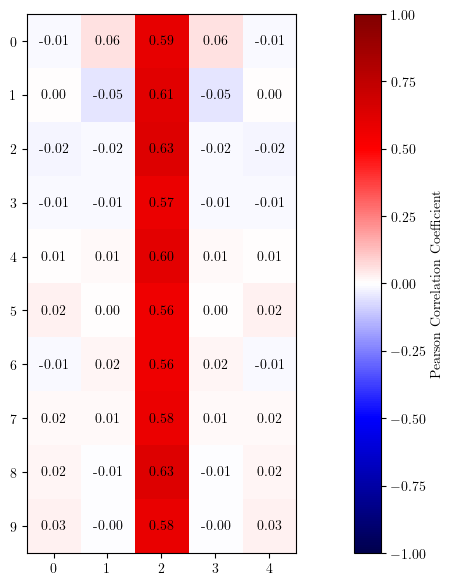
\includegraphics[width = 0.5\textwidth]{Figures/logits_correlation.png}
	\caption{Pearson $r^2$ value for each logit in the ouput of the transition model between $g(s, a)$ and $\ell_r^\mathcal{S}g(\ell_r^\mathcal{S}s,\ell_r^\mathcal{A}a)$, for one of the 675 possible sate action pairs, across 1000 random  seeds for network initialization. }
	\label{fig:logits_correlation}
\end{figure}
Empirically one can see the lack of correlation in Fig.\ref{fig:logits_correlation}, which plots the $r^2$ co-efficient between the transition images across 1000 randomly initialized untrained networks. The network parameterise the next states as two distributions, by outputing an array of 50 logits. As expected, the network responses along the center axis should be invariant to the input transformation. Thus, a positive correlation co-efficient is encouraging. For all other logits in the distribution over the next state there is no evidence of a correlation between the two transition images, at a 5\% significance level.

With the two ouptut's being independent of each other, then correct next state can be selected using the proximal layer reliably, and the networks can be approximately equivariant.



\subsection{CartPole}
A CartPole transition model is a functional approximation to a deterministic Non linear system. In CartPole the transitions between different states in CartPole are governed by the PDEs:
\begin{equation}
	\ddot{\theta} = \frac{g \sin \theta + \cos\theta \left({\frac{-F - m_p l \dot{\theta}^2 \sin(\theta)}{m_c + m_p}} \right )}{l\left ( \frac{4}{3} - \frac{m_p \cos^2 \theta}{m_c + m_p}\right)},
\end{equation}

\begin{equation}
	\ddot{x} = \frac{ F + m_p l (\dot{\theta}^2 \sin \theta - \ddot{\theta} \cos \theta)}{m_c + m_p}.
\end{equation}
Here $g$ is the acceleration due to gravity and is positive, $\theta$ is the angle between the pole and vertical, with the pole length $l$. $F$ is the action force, where the positive direction is right. The masses of the cart and the pole are $m_c, m_p$, respectively. Finally $\dot{}$, indicates a derivative with respect to time.

These PDEs have no closed solution and their form is taken from \cite{florian2007correct} who provides slight corrections to the original dynamics in \cite{barto1983neuronlike}.

To learn this transition model, transitions are sampled from a policy on the MDP, and stored. This is then used as a dataset to perform supervised learning on. The Transition model, $T_\phi: \mathcal{S} \times \mathcal{A} \rightarrow \mathcal{S}$, predicts next states from a state action pair. A state is a vector s:
\begin{equation}
	s = \begin{pmatrix}
		x       \\
		\dot{x} \\
		\theta  \\
		\dot{\theta}
	\end{pmatrix}
\end{equation}
The loss function for the transition model is the average L2 distance between the predicted next state, and the true next state across a batch of samples.
\begin{equation}
	L(\phi) = \frac{1}{N}\sum^N_{(s, a, s')_i \sim \mathcal \tau} ||T(s, a) - s'||_2
\end{equation}
Here $\tau = \{(s, a , s')_1^N\}$ is a batch of transition, of size $N$, sampled from the MDP, and $(s, a, s')$, is the state, action, next state tuple. Often a reward model is required to also make an MDP. For simplicity, the CartPole reward model is used, rather than learned. As such the transition gains a reward of $+1$, if $|\theta| < 12.5^o$, otherwise the episode terminates.

\subsubsection{Constructing Equivariant World Models}
Like in the previous section on \ref{sec:actor-critic}, the equivariant transition models are deep G-CNNs. In contrast to equivariant Actors in the previous section, these networks have to use the proximal pooling layer on their output \ref{sec:proximal_pool}. The equivariance described by these nextworks is to the identity and negative operation, such that;
\begin{equation}
	T(- s, 2*a - 1) =  -T(s, a), \forall
\end{equation}
These transition models, are not truely equivariant but empirically the proximal pooling layer suffices to meet the equivariance condition.

Again in a similar fashion to the actor networks, the transition models have two hidden Group Covolution layers. The input layer for actions also transforms the action from $[0, 1]$ to $[-1, 1]$. Thus the same group convolution layer can be used for both the state and the action input.

\subsubsection{Comparing Convergence of Transition Models}
In order to perform model based RL a transition model must be learnt to simulate transitions, such that the agent can learn a policy that performs better in the original environment. Thus the first set of experiments were training transition models in a supervised learning setting.

Three different pairs of models were trained. The first pair on data collected from an expert and random policy. The second pair took the first dataset and filtered out the transitions which took the right action. The final pair is trained only on data sampled from a random policy.
\begin{figure}
	\centering
	\includegraphics*[width=\linewidth]{Figures/transition_model_cp.png}
	\caption{Transition Model RMS error, plotted against epochs for three different training datasets. Left, the dataset contains a 50/50 split between expert policy sampled transitions, and transitions sampled from a random policy with 80,000 transitions. Center, the same dataset as left, however, with only the left action taken. This dataset contains 40,000 transitions. Right, solely transitions sampled from a random policy, again with 80,000 transitions. All plots have the same set of validation data with a 50/50 split of expert and radom policy sampled data.}
	\label{fig:transition_model_cp}
\end{figure}
In Fig.\ref{fig:cartpole_equivariant_actor} it is clear that the G-CNN despite having the same parameter count, performs substantially better on all 3 datasets. Further, there is a reassuringly stark delta in performance between the equivariant model, and the conventional MLP transition model, when the right action is filtered out. The equivariant model recovers the majority of the performance in this scenario, while the MLP appears to ...

% TODO

\subsection{Catch}
In catch the transitions between states are much simpler with the updates to the ball position between timesteps.
\begin{equation}
	y_{t+1} = y_t + 1.
\end{equation}
And the paddle displacement is goverend by,
\begin{equation}
	x_{t+1} = \text{clip}(1- a_t + x_t, 0, 5).
\end{equation}
Above the clip fucntion, stops the paddle moving beyond the environment's boundaries. The observations from the environment are arrays of shape $5 , 10$, with two ones, indicating the ball and paddle position. The paddle is in row 9, and the ball is only allowed in rows $0 -8$. To encode these constraints the network parameterises two distributions over the ball and paddle locations. The ball can be in one of 45 states, and the paddle may be in one of 5 states. The outputs of the networks are then the logits of the two distributions. In order to predict the next state, the mode of the distributions is taken for both the ball and the paddle. 

Again construction of the G-CNN is much the same as in the case for CartPole, the basic network built from group convolutions. Again two hidden layers are used. Typically for a network predicting distributions against logits, the Binary Cross Entropy loss is used, however, it was found that this was not as effective as using the L2 distance between the logits, and the observation. Thus the loss function to train both transition models was,
\begin{equation}
	L(\phi) = \frac{1}{N}\sum_{(s, a, s') \sim \tau}^N (1 - \delta(\text{done}))||T(s, a) - s'||_2 \end{equation} Here, the one subtlety is that the loss is only back propagated if $s$, is not a terminal state. The indicator function $\delta(\text{done}) = 1 \text{if $s$ is terminal} $. Thus the model only learns transitions goverend by the environment dynamics, and not how to reset the episode.

In order to make the model equivariant the proximal pooling layer a distance metric needs to be used that quantifies how far apart the predictions are. The metric used is an L1 loss between the x, y position in s and s' of both the ball and the paddle. Additionally, to make the possible number of distances greater when the distances are summed, the ball's displacement is multiplied by 0.13. This constant value was found to improve the equivariance behaviour of the proximal pooling layer. The distance metric is then given by,
\begin{equation}
	d(s, s') = ||\text{mode}(T(s, a)_b) - s'_b||_1 + 0.13 ||\text{mode}T(s, a)_p - s'_p||_1.
\end{equation}
The subscripts, $b, p$ indicate the ball and the paddle distributions respectively.

\subsubsection{Comparing Convergence of Transition Models}
In the same manner as before for CartPole, the transition models were trained on three different datasets to asses their convergence behaviour. In the same vein these were a random and expert policy sampled data, only left actions from the previous dataset, and only random policy sampled transitions. 

\begin{figure}
	\centering
	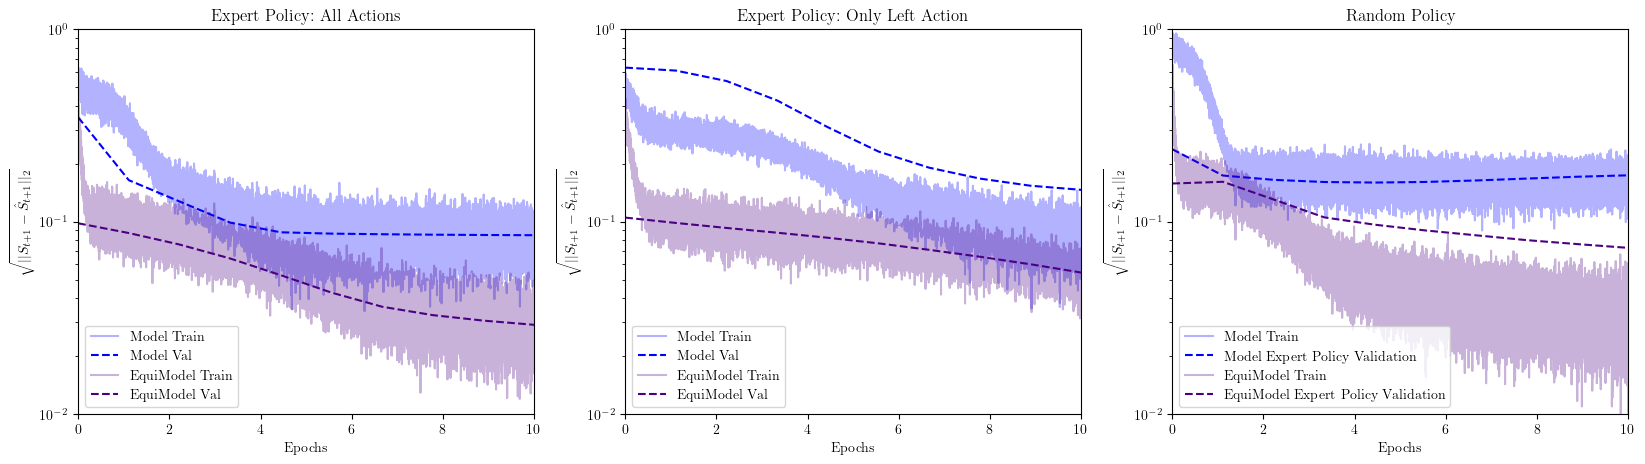
\includegraphics[width=\linewidth]{Figures/transition_model_cp.png}
	\label{fig:transition_model_catch}
	\caption{something}
\end{figure}

\ldots
% TODO: Descriptions and something.



\section{Dyna}\label{sec:Dyna_experiment}
Previously, it was demonstrated that equivariant world models provide advantages over world models without an inductive bias to the symmetries present in the environment.

However, for such techniques to be truly useful, the models must demonstrate an improvement in sample efficiency. This was not the case with the offline trained world models. As the world models required interacting with the MDP many times to create a dataset to learn from. Because of this a set of agents were trained with online learnt transition models in a full Dyna setting, Alg.\ref{algo:Dyna}.

In the same fashion as the Supervised-Dyna agents before, 128 agents were trained at each hyperparameter configuration initialized with independent random seeds. In comparison to the Supervised-Dyna experiments before agents are trained across five planning ratios, $[0.5, 1, 2, 4, 8]$ and $[5, 10, 50, 100]$ Dyna iterations. The planning ratio is the same as before and controls the fraction of time spent planning to acting. The number of Dyna iterations controls the size of the buffer of transitions for both the transition model. To help with reasoning about the training, the size of the replay buffer is,
\begin{equation}
	|\mathcal{D}| = 50000/\text{Num Dyna Iterations}.
\end{equation}
Further, when considering the planning phase, the planning buffer size is related to the acting buffer by the planning ratio,
\begin{equation}
	|\mathcal{D}_p| = \text{PR}|\mathcal{D}|.
\end{equation}
As the number of timesteps is fixed the number of Dyna iterations provides a mechanism for controlling the frequency of planning.
\subsection{Results: CartPole Dyna}
\begin{figure}[h!]
	\centering
	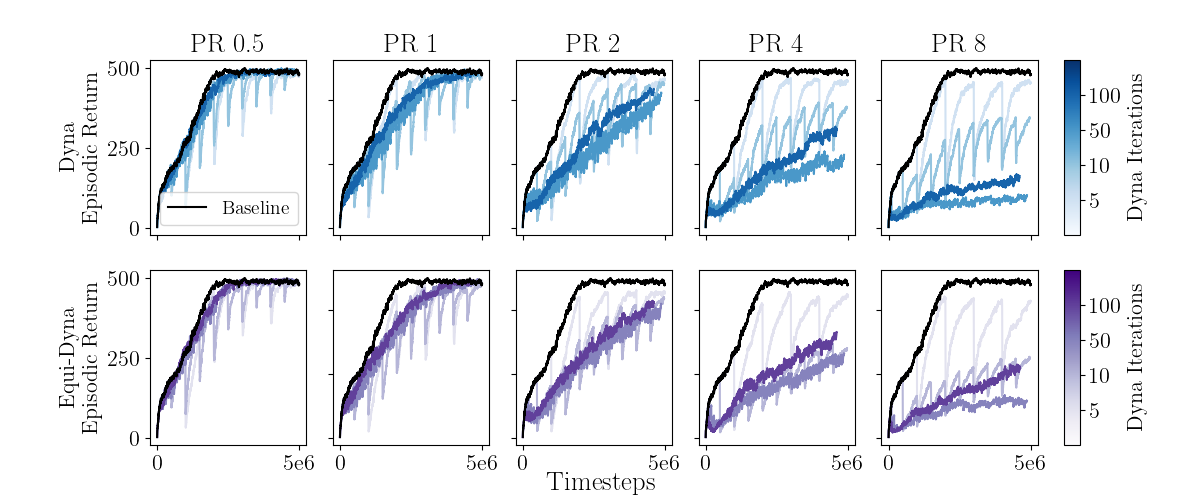
\includegraphics[width=\textwidth]{Figures/dyna_sweep_cp.png}
	\caption{A matrix of plots for mean episodic returns for the CartPole Dyna agents across 128 random seeds
		plotted against number of interaction time-steps in the MDP. The matrix varies planning ratio horizontally, and the top row is the conventional MLP transition model in blue. The equivariant transition models are all on the bottom row, in purple. Each plot contains 5 lines, in black is the baseline actor-critic implementation. The colorbar indicate the number of dyna iterations used to train the agents.}
	\label{fig:cp_dyna}
\end{figure}

The matrix of plots in Fig.\ref{fig:cp_dyna} shows underwhelming performance for the Dyna implementation. Both the Dyna and Equi-Dyna agents underperform the baseline actor-critic in all plots. Further, the model's performance is strikingly similar across all planning ratios and Dyna iterations.

When only considering a planning ratio of 0.5, where the agent learns from twice the number of real transitions as simulated transitions. The agents with higher Dyna iteration count, thus fewer gradient updates\footnote{Batch size is constant, so parameter updates is a function of dataset size.} from simulated transitions, perform similarly to the baseline. Additionally, the discontinuities seen in models with higher Dyna iterations were not present.

These discontinuities are caused by the actor-critic network gaining too much experience in the planning environment. If the planning environment does not simulate the true environment well enough.

The evidence for this is threefold. Firstly such discontinuities, are clearly absent in the expert transition model seen in Fig.\ref{fig:sup-dyna-cp}. Where, the pretrained transition model, has access to more data than is seen by the online trained world models throughout the whole training, and achieves much lower validation loss $0.009$ compared with the lowest transition model training loss across all hyperparameters of $0.039$. This fourfold decrease in loss indicates a far more accurate transition model.

Secondly, considering higher planning ratios it can be seen that the discontinuities are even larger. As higher planning ratios correspond to the actor-critic performing more simulated training. This results in further fitting the actor-critic's policy to the simulated environment. When the agent returns to the true environment the return delta is larger for higher planning ratios, indicating an increasingly negative effect on the policy when performing more simulated training.

Finally, when comparing the higher planning ratios at higher Dyna iterations to lower planning rations. One sees that the majority of policy updates are in the simulated environment, and the transition model learns from a limited amount of simulated data. That the effectiveness of the models collapses in the true environment, emphasizing the inability for the policy learnt predominately in the simulated environment to generalize to the true environment.

The lack of differentiation between both the Dyna agents and the Equi-Dyna agents implies that the same issues are present in both. This is attributed to the poor quality of the online learnt world models. Where the equivariant G-CNN transition model's superior data efficiency and generalization is not sufficient to overcome the limited sample count available for training transition models.

\subsection{Catch}
In comparison to the CartPole environment the Catch environment is a small discrete space discrete and may provide a simpler task for learning.
In the same manner as CartPole, a set of experiments were performed which varied the planning ratio and number of Dyna iterations.
\begin{figure}[h!]
	\centering
	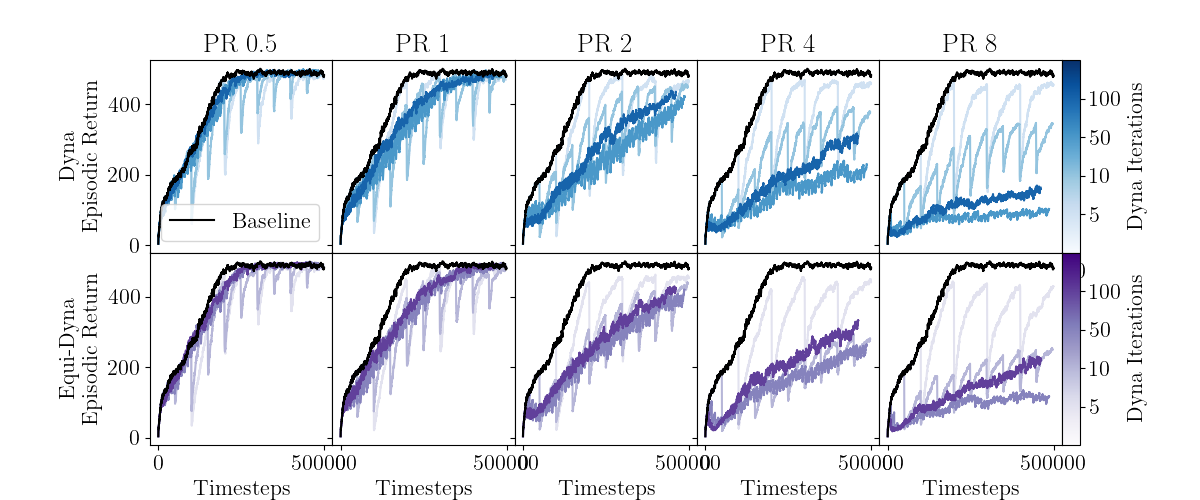
\includegraphics[width=\textwidth]{Figures/dyna_sweep_catch.png}
	\caption{A matrix of plots for mean episodic returns for the Catch Dyna agents across 128 random seeds
		plotted against number of interaction time-steps in the MDP. The matrix varies planning ratio horizontally, and the top row is the conventional MLP transition model in blue. The equivariant transition models are all on the bottom row, in purple. Each plot contains 5 lines, in black is the baseline actor-critic implementation. The colorbar indicate the number of dyna iterations used to train the agents.}
	\label{fig:catch_dyna}
\end{figure}
Despite the small discrete state space, none of the agents were able to improve upon the actor-critic baseline. The similarity, in the patterns shown in the return curves between Catch and CartPole imply that the overfitting to poor simulation is also present.

In the mean returns of the Catch agents over 128 seeds, again minimal difference is seen between the Equi-Dyna agents and the Dyna agents. However, their training dynamics do seem to be similar. At higher iteration count, the return curves are smoother due to a reduced number of updates in the planned environment not allowing the policy to drift from the value learnt in the true environment dramatically. When the planning ratio is increased, the impact upon the quality of the policy is more sever. This degradation is attributed to overfitting the policy to an insufficiently accurate simulated environment.

In comparison to CartPole, the Catch environment only has 675 possible transitions. However, when testing the expert policy and the random policies in Section~\ref{sec:model-based} the joint expert random policy, did not sample every possible state action pair, in 10,000 sampled transitions. When training the agent's world model online from the replay buffer, not all transitions may be present, and the model's inability to generalize to unseen states is still a problem. This poor generalization performance is clear in the return curves as the agent's transition models are not able to produce sufficiently accurate transitions for the policy to learn from.


\section{Conclusion}
In both environment similar behaviour was observed. The Dyna and Equi-Dyna have very comparable performance at the same hyperparameters, which always underperformed the baseline. As such, planning with online models was ineffective.

The poor performance was attributed to transition models that do not deliver sufficient accuracy in producing trajectories that simulate the environment well enough to provide an alternative to samples in the true environment.

The inaccurate transition models suggest providing the models with more data and/or not using the transition model before some point in the training such that enough data can be sampled from the MDP that the transition model can generalize effectively. This However, would not have been straightforward to implement. Implementation constrains of the numerical computing library JAX and available memory, meant that there was no ability to grow array size in code compiled to the XLA backend. This in conjunction with the large memory footprint of thousands of transitions, meant that the workarounds tried with pre allocated replay buffers were infeasible due to out of memory errors on the GPU and RTX 3090.



% \chapter{My First Content Chapter}
\label{chapterlabel2}

% This just dumps some pseudolatin in so you can see some text in place.
\blindtext

% \section{Notes}

\textbf{Definition: MDP Homomorphism} Given some MDP $\mathcal{M}$, where there
exists a surjective map, from $\mathcal{S} \times \mathcal{A} \rightarrow \omc{S} \times
	\omc{A}$. the MDP $\omc{M}$ is an abstract MDP over the new space. The
homomorphism $h$, then is the tuple of $(\sigma, \alpha_s|s \in \mathcal{S})$, where
$\sigma: \mathcal{S} \rightarrow \omc{S}$ and $\alpha_s : \mathcal{A} \rightarrow \omc{A}$.
This surjective map must satisfy two constraints for it to be a valid MDP
homomorphism; \begin{enumerate} \item $R(s, a) = R(\sigma(s), \alpha_s(a))$
	\item $T(s', a, s) = T(\sigma(s'), \alpha_s(a), \sigma(s))$ \end{enumerate}


Rather than learning a tranditional MDP homomorphism, we wish to learn a homomorphic map

$$h: \mathcal{A} \times \mathcal{S} \times \overline{\mathcal{A}} -> \omc{S}$$

With the constraints that the homomorphsim in the simplest case maps of invertersion symmetry $D_2$ where in state space the $D_2$ representtion is $L_2$ and in action space the $D_2$ representaiton is $K_2$. so that $$h(a, s, \overline{a}) = h(K_2 a, L_2 s, \overline{a})$$.

Because we are learning from determinsistic dynamics $T: \mathcal{S} \times \mathcal{A} \rightarrow \mathcal{S}$ and $\overline{T}: \omc{S} \times \omc{A} \rightarrow \omc{S}$ we must also learn that

$$\overline{T}(\overline{s}, \overline{a}) = h(T(s, a), a', \overline{a})$$.

where $overline{s} = h(s, a, \overline{a})$

$$\overline{T}(h(s, a, \overline{a}), \overline{a}) = h(T(s, a), a', \overline{a})$$.


In the case of the cartpole the actions $a, \overline{a} \in [0, 1]$.


\subsection{Training}
The objectiive of training is to use some kind of similarity metric like that used in Approximate MDP Homomorphisms to learn the parametric form of $h$ in a supervised setting, over these (state, action, abstract action, next state) tuples.
With the hypothesis that having a group equivariant network will make the learning more efficient.

% \chapter{General Conclusions}
\label{chapterlabel4}

% This just dumps some pseudolatin in so you can see some text in place.
\blindtext

% \addcontentsline{toc}{chapter}{Appendices}

% The \appendix command resets the chapter counter, and changes the chapter numbering scheme to capital letters.
%\chapter{Appendices}
\appendix
\chapter{An Appendix About Stuff}
\label{appendixlabel1}
(stuff)

\chapter{Another Appendix About Things}
\label{appendixlabel2}
(things)

\chapter{Colophon}
\label{appendixlabel3}
\textit{This is a description of the tools you used to make your thesis. It helps people make future documents, reminds you, and looks good.}

\textit{(example)} This document was set in the Times Roman typeface using \LaTeX\ and Bib\TeX , composed with a text editor. 
 % description of document, e.g. type faces, TeX used, TeXmaker, packages and things used for figures. Like a computational details section.
% e.g. http://tex.stackexchange.com/questions/63468/what-is-best-way-to-mention-that-a-document-has-been-typeset-with-tex#63503

% Side note:
%http://tex.stackexchange.com/questions/1319/showcase-of-beautiful-typography-done-in-tex-friends

% You could separate these out into different files if you have
%  particularly large appendices.

% This line manually adds the Bibliography to the table of contents.
% The fact that \include is the last thing before this ensures that it
% is on a clear page, and adding it like this means that it doesn't
% get a chapter or appendix number.
\addcontentsline{toc}{chapter}{Bibliography}
% Actually generates your bibliography.

\bibliography{bibliography}
\section{Hyperparameters}\label{ap:hyp}
\subsection{Actor-Critic}
All of the hyperparameter choices come from PureJaxRL\cite{alet2021noether}, apart from those for Catch which were slightly modified.
\begin{table}[h!]\label{tab:hyp_ac_cp}
	\centering
	\begin{tabular}{|c|c|}
		\hline
		Hyperparameter  & Value             \\
		\hline
		Optimizer       & Adam              \\
		Learning rate   & 3.5\cdot 10 ^{-4} \\
		Adam: $\beta_1$ & 0.9               \\
		Adam: $\beta_2$ & 0.999             \\
		Adam:$\epsilon$ & 10^{-8}           \\
		Max Grad Norm   & 0.5               \\
		Mini Batch Size & 128               \\
		\hline
	\end{tabular}
	\caption{CartPole Optimizer Hyperparameters}
\end{table}
\begin{table}[h!]\label{tab:hyp_ac_catch}
	\centering
	\begin{tabular}{|c|c|}
		\hline
		Hyperparameter  & Value             \\
		\hline
		Optimizer       & Adam              \\
		Learning rate   & 3.5\cdot 10 ^{-4} \\
		Adam: $\beta_1$ & 0.9               \\
		Adam: $\beta_2$ & 0.999             \\
		Adam:$\epsilon$ & 10^{-8}           \\
		Max Grad Norm   & 0.5               \\
		Mini Batch Size & 10                \\
		\hline
	\end{tabular}
	\caption{Catch Optimizer Hyperparameters}
\end{table}

\begin{table}[h!]\label{tab:hyp_rl}
	\centering
	\begin{tabular}{|c|c|}
		\hline
		Hyperparameter      & Value \\
		\hline
		PPO:Clip-$\epsilon$ & 0.2   \\
		Value coefficient   & 0.5   \\
		Entropy coefficient & 0.01  \\
		Update length       & 128   \\
		Discount: $\gamma$  & 0.99  \\
		GAE-$\lambda$       & 0.95  \\
		\hline
	\end{tabular}
	\caption{RL Hyperparameters}
\end{table}

\begin{table}[h!]\label{ap:parm}
	\centering
	\begin{tabular}{|c|c|}
		\hline
		Network                  & Parameter Count \\
		\hline
		Actor-Critic             & 9155            \\
		Symmetrizer              & 9155            \\
		Equivariant Actor-Critic & 8961
		\hline
	\end{tabular}
	\caption{Actor-Critic network parameter Counts}
\end{table}

\subsection{Transition Model}
\begin{table}[h!]\label{tab:hyp_tm}
	\centering
	\begin{tabular}{|c|c|}
		\hline
		Hyperparameter  & Value           \\
		\hline
		Optimizer       & Adam            \\
		Learning rate   & 1\cdot 10 ^{-3} \\
		Adam: $\beta_1$ & 0.9             \\
		Adam: $\beta_2$ & 0.999           \\
		Adam:$\epsilon$ & 10^{-8}         \\
		Max Grad Norm   & 0.5             \\
		Mini Batch Size & 64              \\
		\hline
	\end{tabular}
	\caption{Transition Model Hyperparameters}
\end{table}

\section{CartPole}
\subsection{Transition Distribution By Angle}
\begin{figure}[h!]
	\centering
	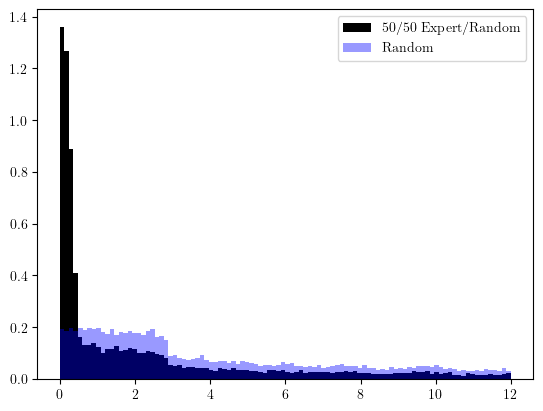
\includegraphics[width=\textwidth]{Figures/angles_cp.png}
	\caption{Histogram plot of transitions initial state against absolute angle. 50/50 Expert/Random refers to the joint expert-random dataset. }
	\label{ap:dist_cp}
\end{figure}

\subsection{Supervised-Dyna}

\begin{figure}[h!]
	\centering
	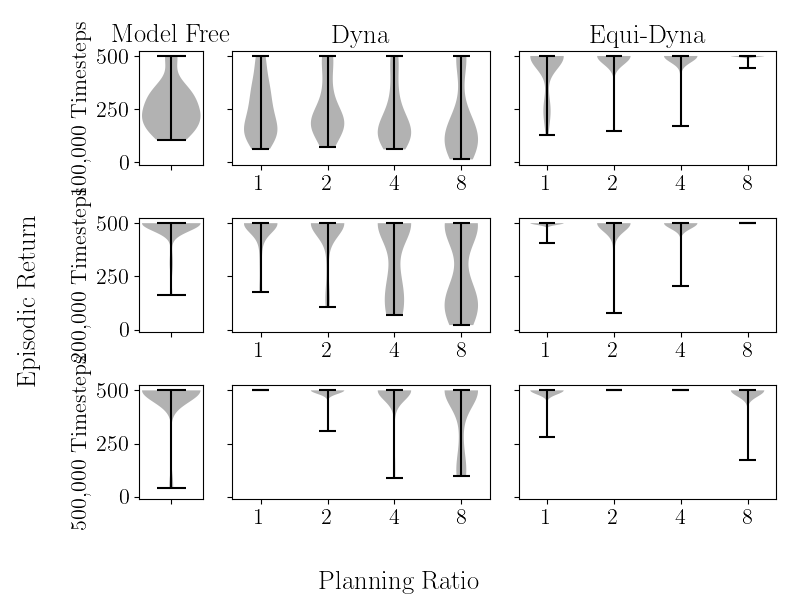
\includegraphics[width=\textwidth]{Figures/violin_cp_expert.png}
	\caption{Violin Plot of episodic returns at timestep intervals across all tested planning ratios on the CartPole environment.}
\end{figure}

\begin{figure}[h!]
	\centering
	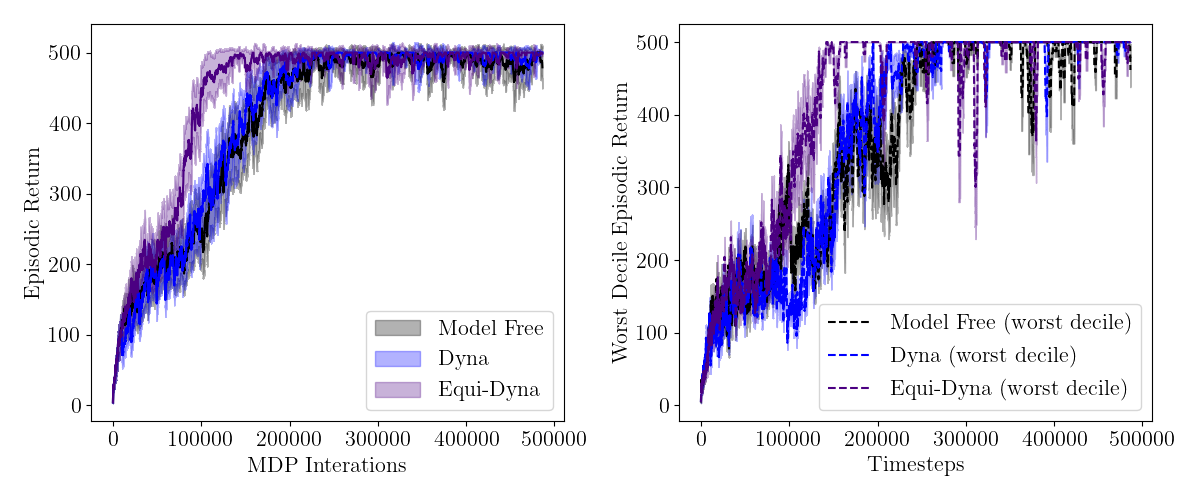
\includegraphics[width=\textwidth]{Figures/Expert_dyna_cp_pr1.png}
	\caption{Episodic returns for Supervised-Dyna agents with a baseline on the CartPole environment. Using a planning ratio of one.}
\end{figure}
\begin{figure}[h!]
	\centering
	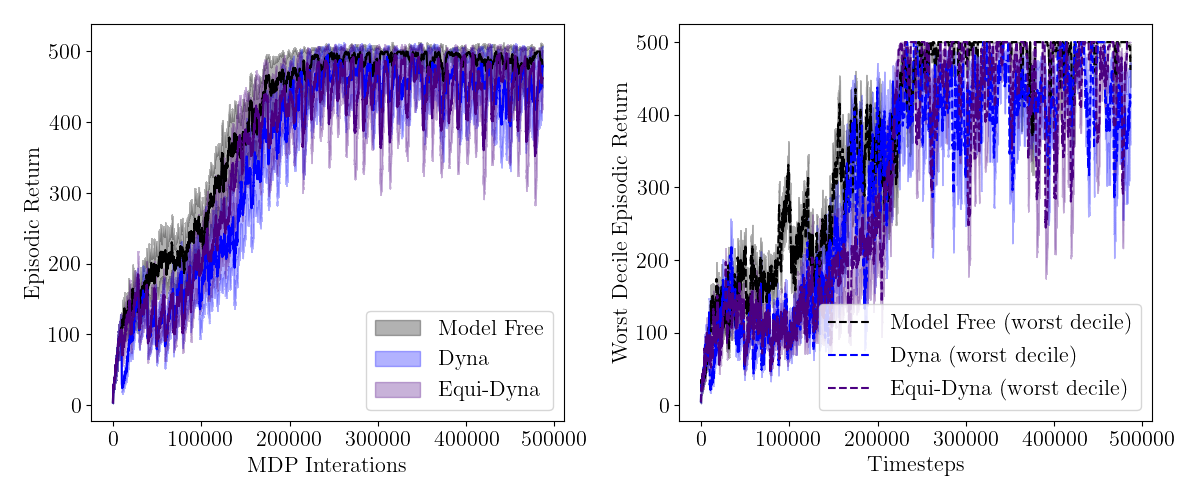
\includegraphics[width=\textwidth]{Figures/Expert_dyna_cp_pr2.png}
	\caption{Episodic returns for Supervised-Dyna agents with a baseline on the CartPole environment. Using a planning ratio of two.}
\end{figure}
\begin{figure}[h!]
	\centering
	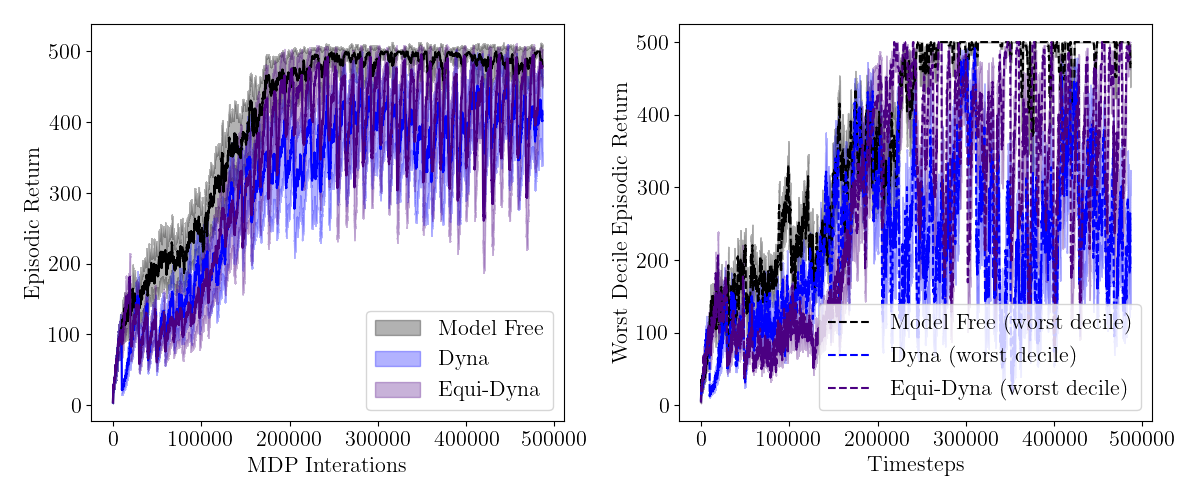
\includegraphics[width=\textwidth]{Figures/Expert_dyna_cp_pr4.png}
	\caption{Episodic returns for Supervised-Dyna agents with a baseline on the CartPole environment. Using a planning ratio of four.}
\end{figure}
\begin{figure}[h!]
	\centering
	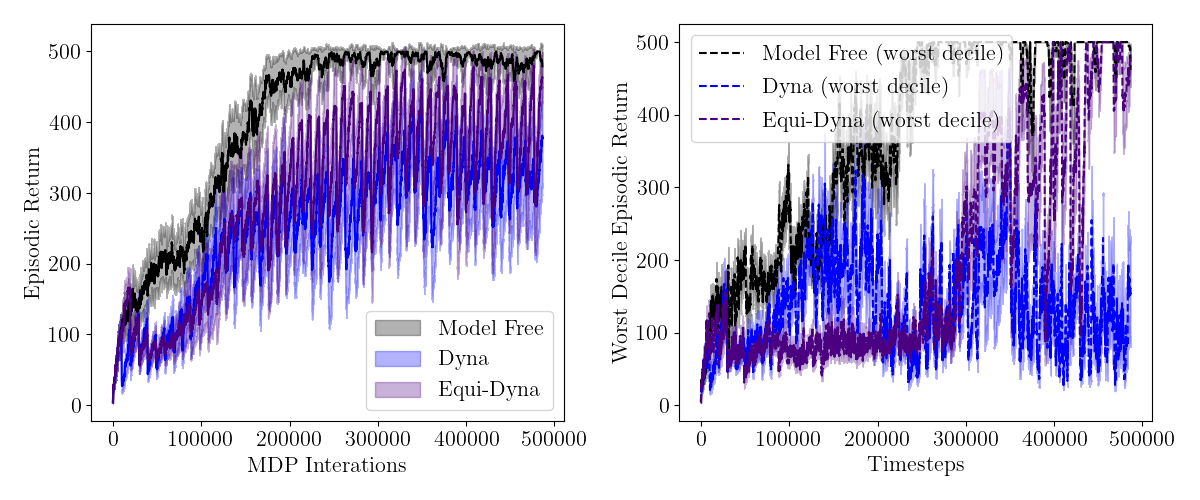
\includegraphics[width=\textwidth]{Figures/Expert_dyna_cp_pr8.png}
	\caption{Episodic returns for Supervised-Dyna agents with a baseline on the CartPole environment. Using a planning ratio of eight.}
\end{figure}

\newpage

\section{Catch}



\subsection{Supervised-Dyna}\label{ap:supervised-dyna-catch}

\begin{figure}[h!]
	\centering
	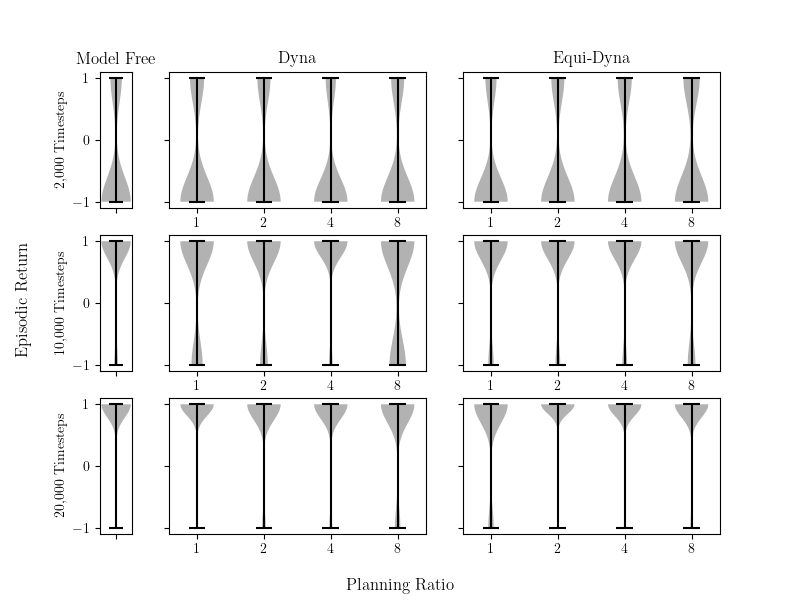
\includegraphics[width=\textwidth]{Figures/violin_catch_expert.png}
	\caption{Violin Plot of episodic returns at timestep intervals across all tested planning ratios on the catch environment.}
\end{figure}

\begin{figure}[h!]
	\centering
	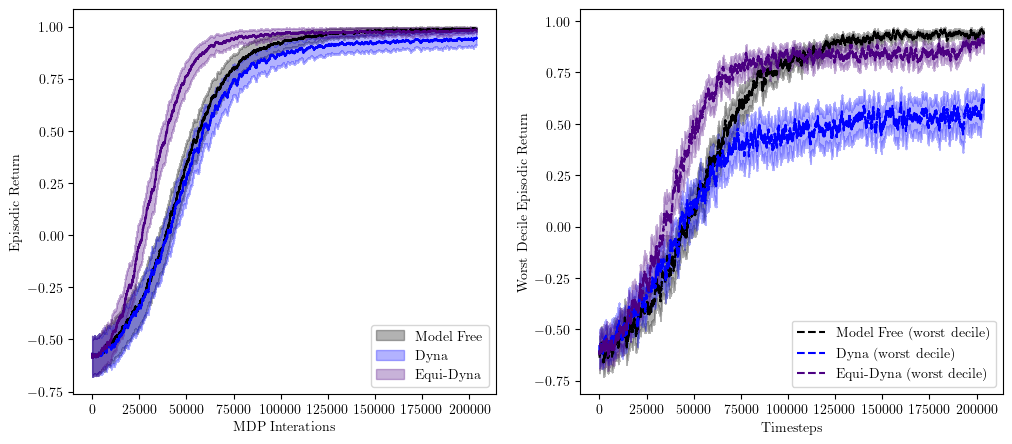
\includegraphics[width=\textwidth]{Figures/Expert_Dyna_Catch_pr1.png}
	\caption{Episodic returns for Supervised-Dyna agents with a baseline on the Catch environment. Using a planning ratio of one.}
\end{figure}
\begin{figure}[h!]
	\centering
	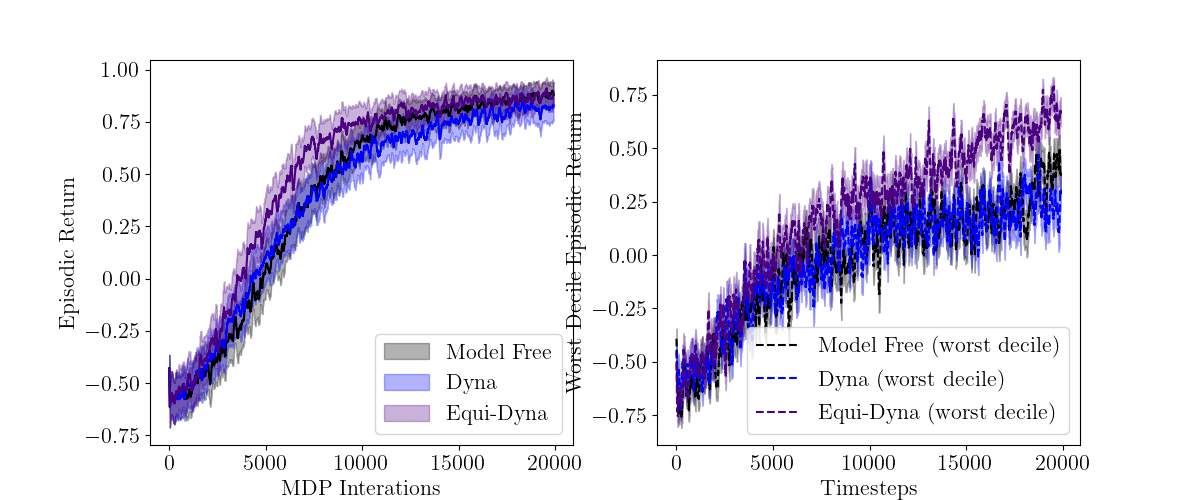
\includegraphics[width=\textwidth]{Figures/Expert_Dyna_Catch_pr2.png}
	\caption{Episodic returns for Supervised-Dyna agents with a baseline on the Catch environment. Using a planning ratio of two.}
\end{figure}
\begin{figure}[h!]
	\centering
	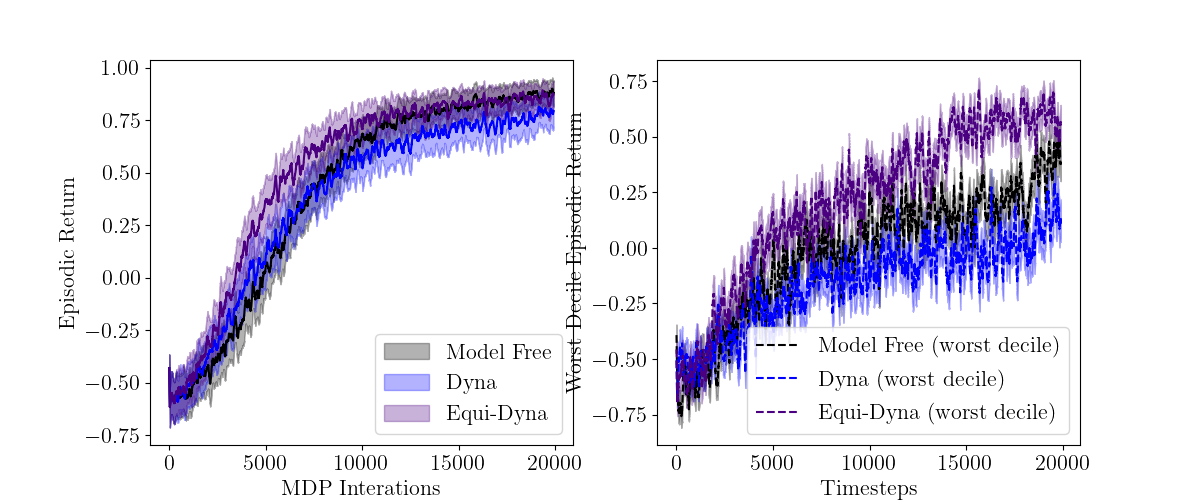
\includegraphics[width=\textwidth]{Figures/Expert_Dyna_Catch_pr4.png}
	\caption{Episodic returns for Supervised-Dyna agents with a baseline on the Catch environment. Using a planning ratio of four.}
\end{figure}
\begin{figure}[h!]
	\centering
	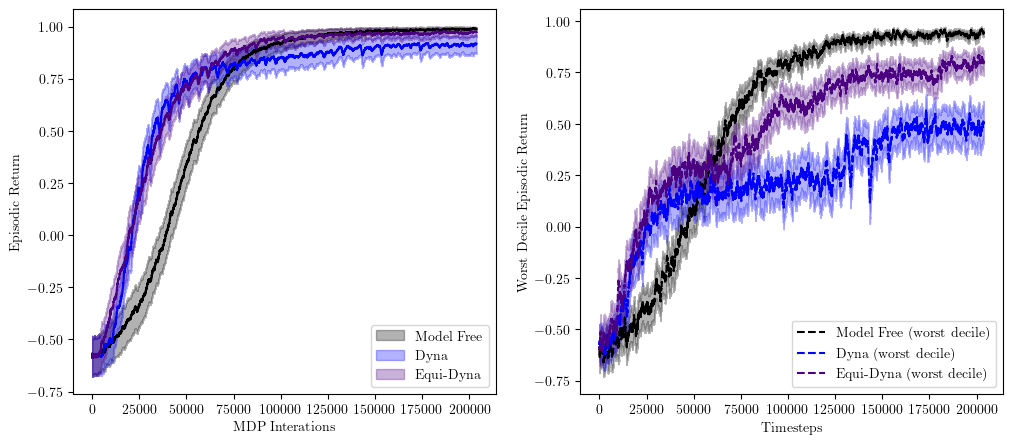
\includegraphics[width=\textwidth]{Figures/Expert_Dyna_Catch_pr8.png}
	\caption{Episodic returns for Supervised-Dyna agents with a baseline on the Catch environment. Using a planning ratio of eight.}
\end{figure}

% All done. \o/
\end{document}
